\chapter{Access point clustering}
%To enable collaborative channel allocation, it is
%important for every AP to know which APs it is collaborating with.
%One way to share information about who collaborates with who,
%is to let the access points group together. Information relevant for channel
%allocation can then be shared freely within the group, between APs.

%We will proceed by looking at some of the requirements for a group creation algorithm.
%It should work decentralized in a distributed fashion. Hence, not only does the APs have to
%be imposed group membership, but they also have to be able to create and definine
%meaningful groups on their own. Later we will propose an algorithm to create groups,
%and then evaluate computed groups based on the algorithm.


\section{Introduction}
While it at first sounds incredibly desirable to let the entire population of for instance New York's access points organize themselves in an optimal channel-plan,
at second thought the idea may prove to be a little ambitious. Being limited by the NP-complete nature of DSATUR or similar graph coloring algorithms
we have to set some reasonable constraints on the size of the \textit{collaborating group}. The amount of nodes that will collaborate on the problem of finding an optimal channel distribution
plan may not need to be very high.

Let us for a moment look at an ideal example: a city that only consists of small apartment buildings that are entirely isolated from interference produced in external networks.
How could we build a group in such a case? Turns out it is not that hard. Each access point would be able to collaborate with every other observable access point.
When computing channel distribution there would be no risk of surpassing the viable amount of nodes to compute the distribution for, as the group is limited to the apartment building. Sadly for us the world is not ideal,
and it is not impossible that every access point in New York can observe eachother through a transitive relation. This means the size of
the collaborating group would be vast and completely unviable.  

This does not mean that creating reasonably sized groups of access points is impossible, but it poses a more difficult challenge. 
We need to filter out redundant nodes to create an approximated version of the ideal example.

Having a picture of the typical cityscape in mind, we know that buildings are naturally
separated by streets, bridges, parks, and so on. Rural areas are similar, but networks are spaced more unevenly
and usually only affecting each other in one plane.

Remembering attenuation, we know that RF-interference is also a property of distance. 
These pieces of information tells us that RSSI readings between access points in two separated buildings should be lower than readings between access points in adjacent apartments.
In the following chapter we will consider how we can utilize the RSSI readings between access points to build a clustering algorithm that creates reasonable groups of access points. 

%The should consist of APs that interfere with each other when their channels are overlapping, so that overlap can be avoided with a channel allocation algorithm run within the group. Not all APs in
%the connected group will necessarily be able to hear each other on the radio directly, but all nodes
%should be able to hear each other through a transitive relation (neighbour of a neighbour, etc.).

\section{Problem overview}
The main problem we are dealing with is finding a way for access points to group together in clusters that are geographically close to each other. This can either be solved with a centralized
coordinator or with a peer-to-peer distributed protocol. In this thesis we will be focusing on the distributed approach, but first we will take a look at the pros and cons of each approach.

\subsection{Centralized model}
Let us briefly envision how a centralized model might look. As we want to propose a solution that works across private consumer networks as well as larger corporate networks,
we can not assume that all networks are under the same administrative domain. This is where the centralized approach is limited, and why most solutions presented in the related work section is usually only deployed under the same extended service set (ESS).

Just like a distributed version, a centralized controller is also restricted by the NP-complete nature of all graph colouring algorithms.
To be able to compute a channel plan using heuristics, it has to identify groups of nodes that impacts each other severely. 

The advantage of the centralized model is the ability to have the full picture of access points readily available. Let us assume the controller is placed at an ISP or a router manifacturer.
The controller could potentially know exactly where in the world the access points are placed. Creating groups would be as simple as dividing within naturally separative geographical barriers like roads, streets and buildings. 

For a central controller to be able to identify APs that are near eachother and compute the optimal channel distribution, APs need to report their radio readings to the controller. 
The controller then needs to identify which of all the observed APs it can control, and which is not controllable and has to be treated as noise. There would be no requirement for
communication in between nodes, which reduces complexity a lot.  

A major drawback of the centralized approach is that nodes that are near eachother have to be under the same controller. If there are too many nodes around
that can not be controlled by the controller, all nearby access points would be treated as noise and regular channel allocation schemes would have to be applied.
Even though in there is a tendency for apartments in the same building to have the same ISP in Norway, there is no gurantee for that to always be the case.  

\subsection{Distributed approach}
We will continue considering a distributed approach as the main topic of the thesis. In reality this idea has some major challenges that we have to overcome. Here are the most prominent ones: 
\begin{enumerate}
	\item The group creation itself. Based on the RSSI-readings and the communication channel, nodes have to be able to organize themselves in a tight cluster of nodes that
		includes all nodes that impacts each other most severely. This problem essentially boils down to a clustering problem. This is the main issue we will
		try to find a reasonable solution for. 
	\item The communication channel. Nodes have to be able to communicate with eachother. The 802.11 standard describes no protocol for communication between access points that are not on the same extended service set. This communication would have to happen on the network layer, preferably over TCP. This communication channel would have to convey a messages that enables group creation,
		most likely a custom protocol. 	
	\item State synchronization. As all nodes have to compute a channel plan for the group, they all need to have synchronized information about the members of the groups
		and possibly also every other node's RSSI-readings. 
	\item Channel plan computation. Even though the centralized approach would have a similar problem, it will be more difficult to solve in a distributed fashion as 
		it is reasonable to assume that an access point has limited computational power. This point extends past the scope of the thesis, but algorithms like DSATUR {{(insert ref)}}
		and SCIFI are examples of algorithms that computes channel plans as a graph colouring problems.
\end{enumerate}

\section{Computation assumptions and requirements}
Moving forward in the next chapters we will be looking at possible ways for nodes to organize themselves into groups.
We will be using the data we fetched in chapter \ref{dataacc}. The data provides a topology of nodes where all nodes have a list of neighbouring nodes.
This neighbour list contains the appropriate computed RSSI-readings for each node. Based on the RSSI-values of their neighbours, the nodes should be able to create groups that resembles
clusters. It is important that the border between two different groups are placed in such a way that interference between the two groups are as minimal as possible. To simplify the computation procedure and to reduce the workload for building the simulation program we are going to to a number of assumptions. 

    \begin{enumerate}
    \item Assumption 1: All nodes involved in the simulation also runs the group creation algorithm. 
		\item Assumption 2: When a node is observed over radio, it is also known how to directly contact the node (e.g. via TCP). This assumption also implies that there is implemented a protocol that lets nodes communicate and exchange information about their RSSI-readings and group membership. For now we will assume this is true, but in chapter {{(ref)}} we will address the issue. 
		\item Assumption 3: All nodes in a group are completely synchronous, and always have an equal image of the state of the group at a given time. Sharing information with the group is instant. This is also an issue that will be addressed in chapter {{3}}.
    \end{enumerate}
\section{Program design}
\subsection{Design choices}
The program is designed to be modified so it can accomodate different algorithm types without changing the fundamental framework.
Everything regarding group computation is implemented in Python 3 \cite{Python3}, and is designed parse the output from the data generation program and use it directly.
Group computation should be a fast operation, while the data generation (or fetching) is a slow process and should only be done once every time a new data set is required.
The program is not parallelized to keep results consistent and to easier debug and locate program errors. 

\subsection{Group framework}
The group framework consists of 3 classes with different responsibilities:
\begin{itemize}
	\item \textbf{Group}. An object of this class is an abstraction of all the nodes that belong to the same group. Because we assumed that all nodes have equal
	information about group membership and RSSI-readings, we can store all the members of each group in a list and let the group object act as a unified entity on
	behalf of the entire group. All the interfaces and logic for forming groups is placed within this class. A method named \verb|iteration|
	has the responsibility of triggering the appropriate action based on the state of the group. For instance adding nodes, removing nodes or merging the group
	with another. This is the part of the code that has to be changed when implementing and changing algorithms. If an action was performed the method returns 1, else it returns 0. 

	\item \textbf{GroupCollection}. An object of this class contains all the groups used in a simulation. Its main functional responsibility is looping through all the groups
	and calling the \verb|iteration| method of each group once. This is done in the GroupCollection's \verb|iterate| method. It accumulates the amount of changes done in all the groups,
	by adding the return values of the Group object's \verb|iteration| method. It also handles the destruction of groups, and bootstrapping of newly created groups.

	\item \textbf{Simulation}. An object of this class handles the bootstrapping of groups, where all nodes (given in the input file) are parsed and
	put in their own grown group. Consequently, at the beginning of each computation the amount of groups is equal to the amount of nodes.
	The Simulation class is also responsible for starting and stopping the simulation itself. After bootstrapping all the groups, the Simulation enters a loop
	where it calls the \verb|iterate| method in the GroupCollections object once every run. All the groups have converged and reached a steady state 
	once the amount of changes returned by the GroupCollection's \verb|iterate| method is equal to zero. The results are written to file.
\end{itemize}
{{flowchart}}
\subsection{Output file structure}
The results of the group computations are writen to file. The results does not only contain the resulting divison of groups, but to be able to recreate the simulation
visually, the results contains the topology of all nodes and their group membership for each iteration in the simulation process. This means that we can step-by-step
recreate the simulation. The data is stored as JSON, and the structure can been seen in figure \ref{fig:jsongroup}.
Having the data stored as JSON means that the data is language independent. This allows us to either implement a parser in python for the data and use \verb|matplotlib| to visualize it,
or we can use another applicaton to visualize the data. Since we already have the topology visualizer
written in HTML and JavaScript from chapter \ref{dataacc}, we can extend this program to let us upload a group creation output file. 
\begin{figure}[H]

\begin{minipage}{\linewidth}
\begin{lstlisting}[language=json]
  "iterations": {
    "0": {
      "0": {
	"groupName": "GROUP0",
        "members": {
          "0": "NODE0"
	},
	"memberCount": 1
    },
      "1": {
	"groupName": "GROUP1",
	"members": {
	  "0": "NODE1"
	},
	"memberCount": 1
      }
  },
    "1": {
      "0": {
	  "groupName": "GROUP1",
	  "members": {
	    "0": "NODE0",
	    "1": "NODE1"
	},
	"memberCount": 2
     }
  }
}
\end{lstlisting}
\end{minipage}

\caption{Group simulation file structure}
\medskip
\small
This particular simulation had two iterations. In the first iteration there were two groups, each with one member node. In the second iteration the two groups has merged to one group, now
containing both nodes. 
\label{fig:jsongroup}
\end{figure}



%\section{Algorithms}\label{algorithm}
%We will consider three possible approaches to cluster access points. First we will look at a minimal and basic approach without any complicated heuristics or algorithms. 
%Next we will consider a well known clustering algorithm and treat the problem as a pure clustering problem. Finally we will look at the problem as a graph partitioning problem.
%All approaches will be tested with the same topologies: one uniformly distributed, one used for evaluating traditional clustering algorithms, and two topologies 
%of towns fetched from Wigle. Henceforth we will for the sake of simplicity be referring to APs that are running the group algorithm as \textit{nodes}.

\section{Creating groups with clustering}
In this section we will consider and evaluate a way to divide access points in groups.

\subsection {Agglomerative Clustering}
\subsubsection{Description}
Agglomerative clustering  \cite{agglomerative} is a variant of hierarchical clustering where clusters are pairwise greedily merged. The starting number of clusters is the same as the number of
points in the data set. Based on a specified distance metric, the two clusters that are closest to one another is merged into combined cluster. The clustering is complete
when there is only one cluster left. It falls under the category of hierarchical clustering, and a dendrogram is iteratively being built for each merge,
containing all past merges of the clusters. An example of agglomorative clustering can be seen in {{figure}}\ref{fig:agglomerative}.

\subsubsection{Evaluation}
Agglomerative clustering provides us with the basic idea for a an algorithm we can use to create access point groups. However, there are two points where agglomerative clustering
fails to meet our requirements: 
\begin{itemize}
	\item There is no upper limit to the amount of nodes in each cluster
	\item As the clustering algorithm will be running distributed  on each cluster, a decision has to be made with only the local distance observations at hand.
		Assuming that there exists two groups that finds each other the closest (most disturbing), might prove a fallacy. RSSI is observed locally, and while one node observes another with a given signal strength,
		the mututal observation might be a different one. This could create a deadlock where there exists no combination of group pairs where both observes the other
		as the closest group. 
\end{itemize}

The first point has the trivial solution of checking the number of nodes before accepting a merge,  and would only be a slight implemention change of agglomorative clustering. 
The second point forces us to change the paradigm of always finding two mutually closest groups. 

\subsection{K-Nearest Neighbour Clustering}
\subsubsection{Description}
To resolve the problems discussed in the previous section, we will suggest a slighly different algorithm and refer to it as K-Nearest Neighbour Clustering. 
In this method, similar to agglomerative clustering, in the beggining there are equally many clusters as there are nodes. Instead of looking for pairs that are mutually close,
each cluster seeks to merge with the cluster that is closest. The distance is defined by the distance metric. The merge will always happen as long as the resulting cluster does 
not contain a higher node count than K.

\subsubsection{Distance metric}
The distance metric lets us specify exactly what the distance between two clusters signifies. As each cluster usually consists of several nodes, there are multiple
options for what the distance between two clusters could be defined as. The distance metrics used in hierarchical clustering are typically either
\begin{itemize}
	\item The average distance between the nodes of each cluster
	\item The minimum distance between the nodes of each cluster
	\item The maximum distance between the nodes of each cluster
\end{itemize}

The metric we will use is the -dBi value of neighbouring nodes. Every node in a cluster tracks the observed -dBi value of all other nodes that are not a member of the cluster.
The cluster containing the node with the highest -dBi value will be merged together with original one. This is similar to the minimum distance metric. 

\subsubsection{Implementation}
Each node begins by identifying itself as a member of a group that only contains itself.  Let us call this group $a$.
Group $a$ loops throught the radio readings of every member of the group, and picks the node with the highest observed -dBi value
to contact. In the beginning there is only one node in group $a$. Hence in the first iteration this node's radio readings alone will decide which group to merge with. 
The neighbour node, which we will call $B$, is the node that disturbs group $a$ the most. $B$ is a member of group $b$.
In other words, group $a$ wants to merge with group $b$ to create a larger group that contains node $B$.

A merge happens in the following way: the members of the two groups exchange information about all their member nodes and their radio readings and combine the information.
As the data is now identical for all the members of both groups and they can make identical choices it means that they are part of the same group. 

In our simulation this is as easy as combining two Group objects into one. A pseudocode sample of an implementation can be seen in \ref{fig:groupmerge}.
In a real world implementation there would have to be a supporting protocol to 
enable the flow of information and synchronization of data. These specific challenges will be addressed in chapter {{insert chapter}}.

	\begin{figure}[H]
		\tiny
		\begin{python}
allGroups = [];
K = 120;

for node in topology: //Initialize groups
	g = new Group()
	g.members.append(node)
	allGroups.append(g);

while True: //Run as long as there are changes
	changes = 0;	
	for group in allGroups: 
		globalMaxDbi = -INFINITE
		globalClosestNode = None

		for node in group:
			localMaxDbi = -INFINITE
			localClosestNode = None

			for neighbour in node.neighbours:
				if neighbour.dbi > localMaxDbi:
					localMaxDbi = neighbour.dbi
					localClosestNode = neigbour

			if (localMaxdbi > globalMaxDbi):
				globalMaxDbi = localMaxDbi
				globalclosestnode = localclosestnode:

		var groupToMergeWith = globalclosestnode.group
		if (length(group.members) + length(groupToMergeWith.members)) < K:
			var newGroup = new Group()
			newgroup.members = group.members + mergeWith.members
			allGroups.append(newgroup)
			allGroups.remove(mergeWith)
			allGroups.remove(group)
			changes = 1
	if (changes == 0):
		break
		\end{python}
			\caption{Pseudocode sample of how the K-Nearest Neighbour Clustering runs in a simulated environment}
			\label{fig:groupmerge}
	\end{figure}



We can not always accept merges, else we would end up with a group that spanned the entire topology. That is why we define a maximum threshold for the amount of members a group can have, 
referred to as K. If the sum of members in two groups that wants to merge exceeds K, the merge is aborted and no changes is reported to have happened for either group. 
This means that the simulation algorithm converges when no groups remain that are small enough to merge with another.
 
\subsection{Results of on different topologies}
Figure \ref{fig:knearest}a shows the result of running the K-Nearest Neighbour Clustering algorithm on a uniform distribution topology, while figures \ref{fig:knearest}b, \ref{fig:knearest}c, \ref{fig:knearest}d shows the resulting clusters after running it on topologies on citites and towns collected by WiGLE. The different node colors indicate different group memberships.
%\begin{figure}
%	\begin{minipage}
%		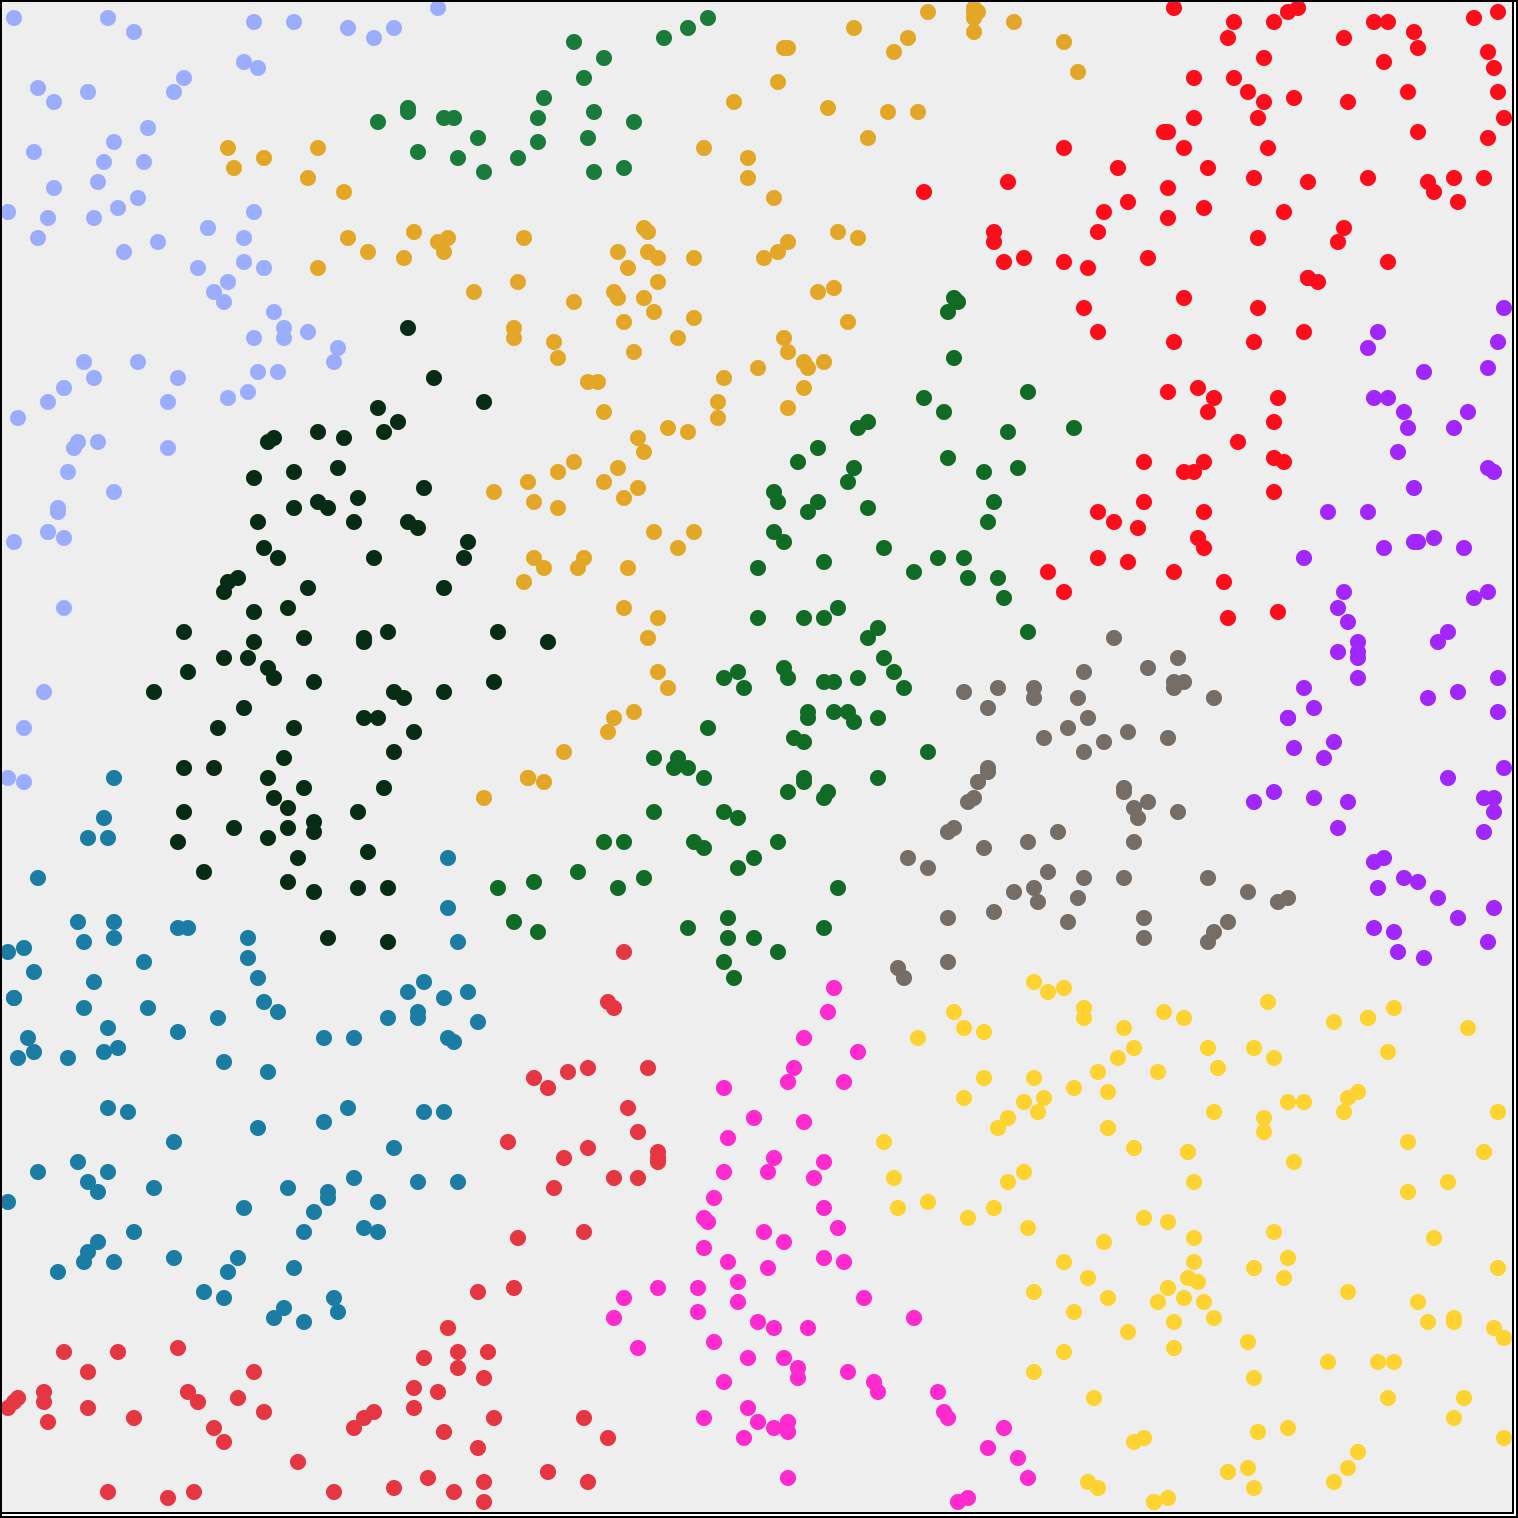
\includegraphics[width=.8\linewidth]{Images/computations/BASIC500x500_1000n.jpg}
%		\caption{A}
%		\label{fig:basic_uniform}
%	\end{minipage}
%
%	\begin{minipage}
%		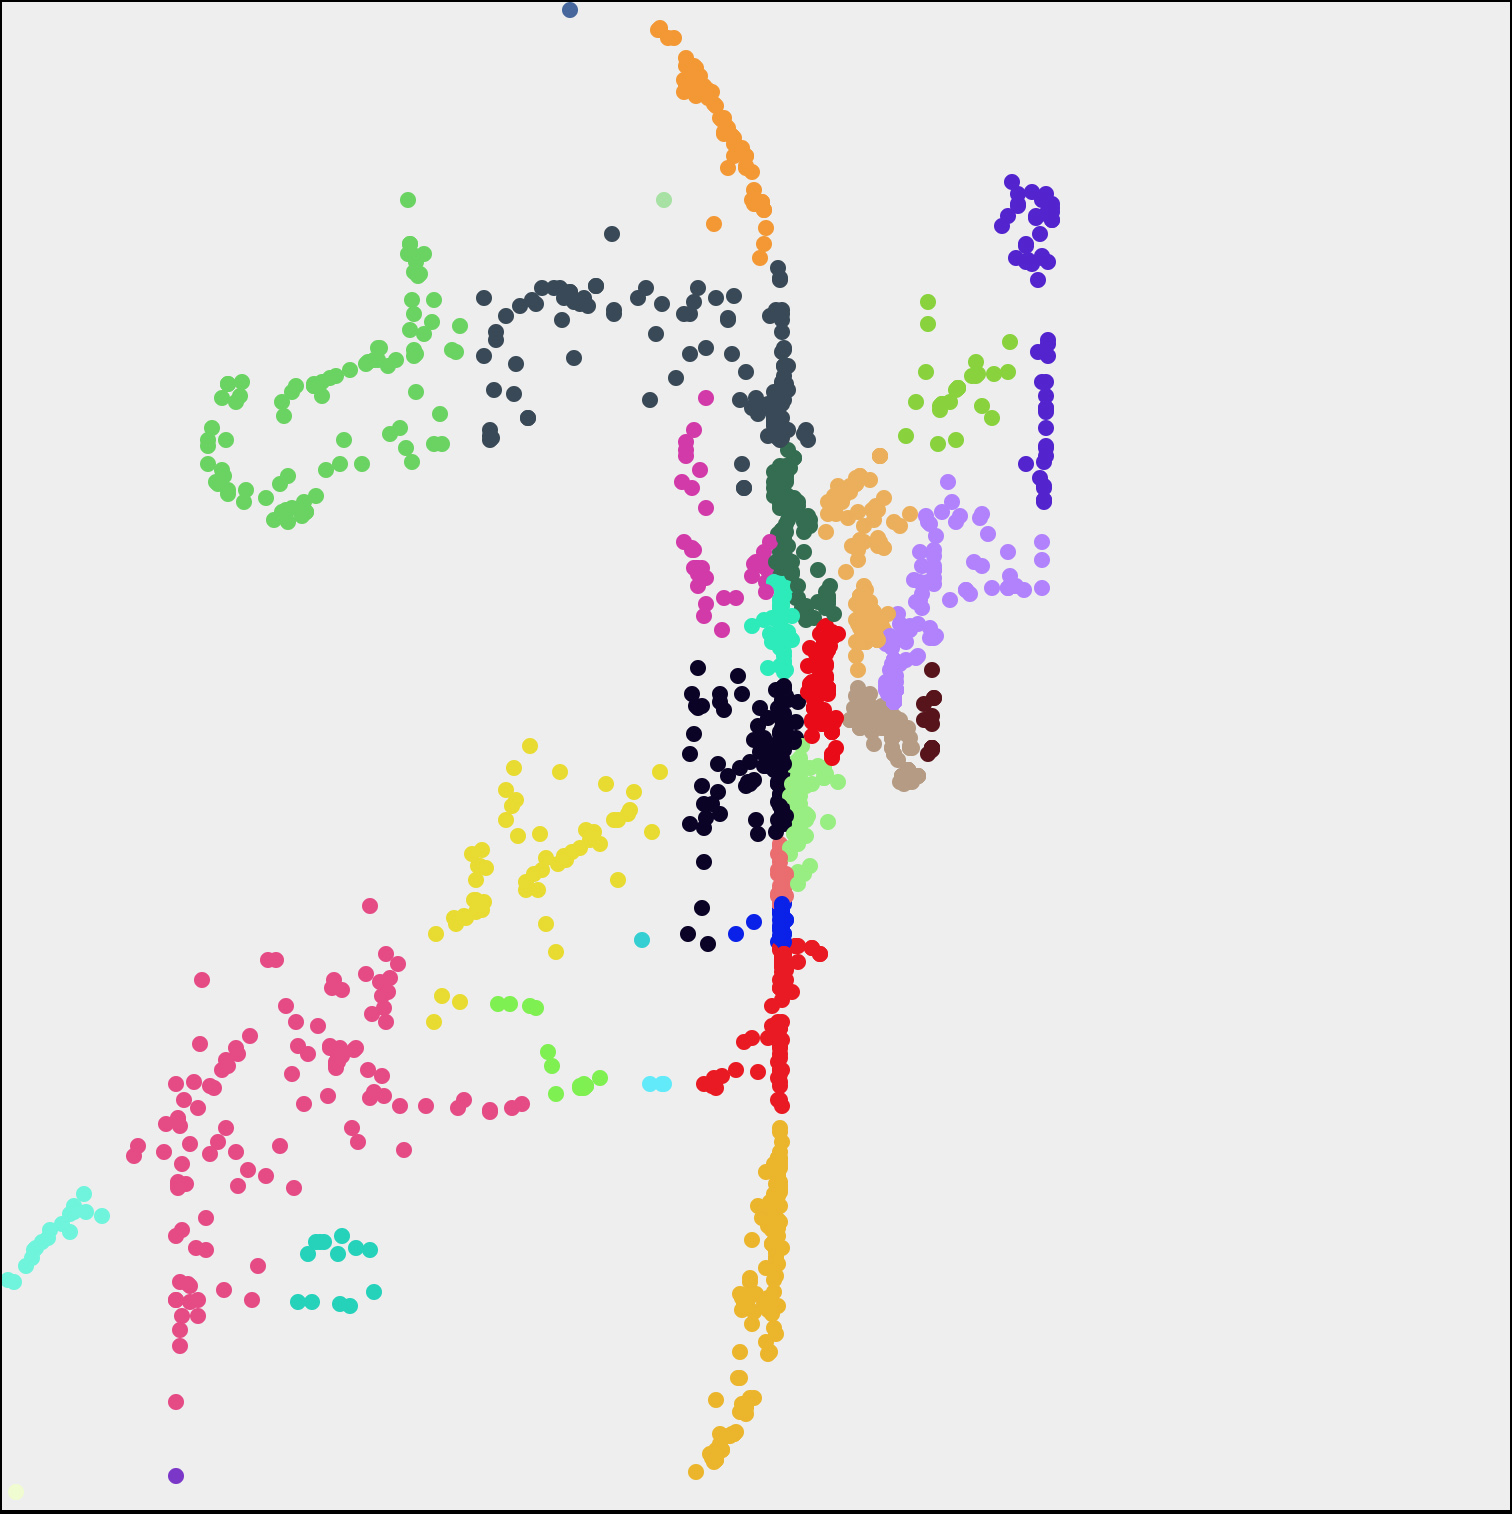
\includegraphics[width=.8\linewidth]{Images/computations/BASICForks.jpg}
%		\caption{B}
%		\label{fig:basic_forks}
%	\end{minipage}
%\caption{plots of....}
%\label{fig:fig}
%\end{figure}
\begin{figure}
		\centering
		\subfloat[Uniform]{{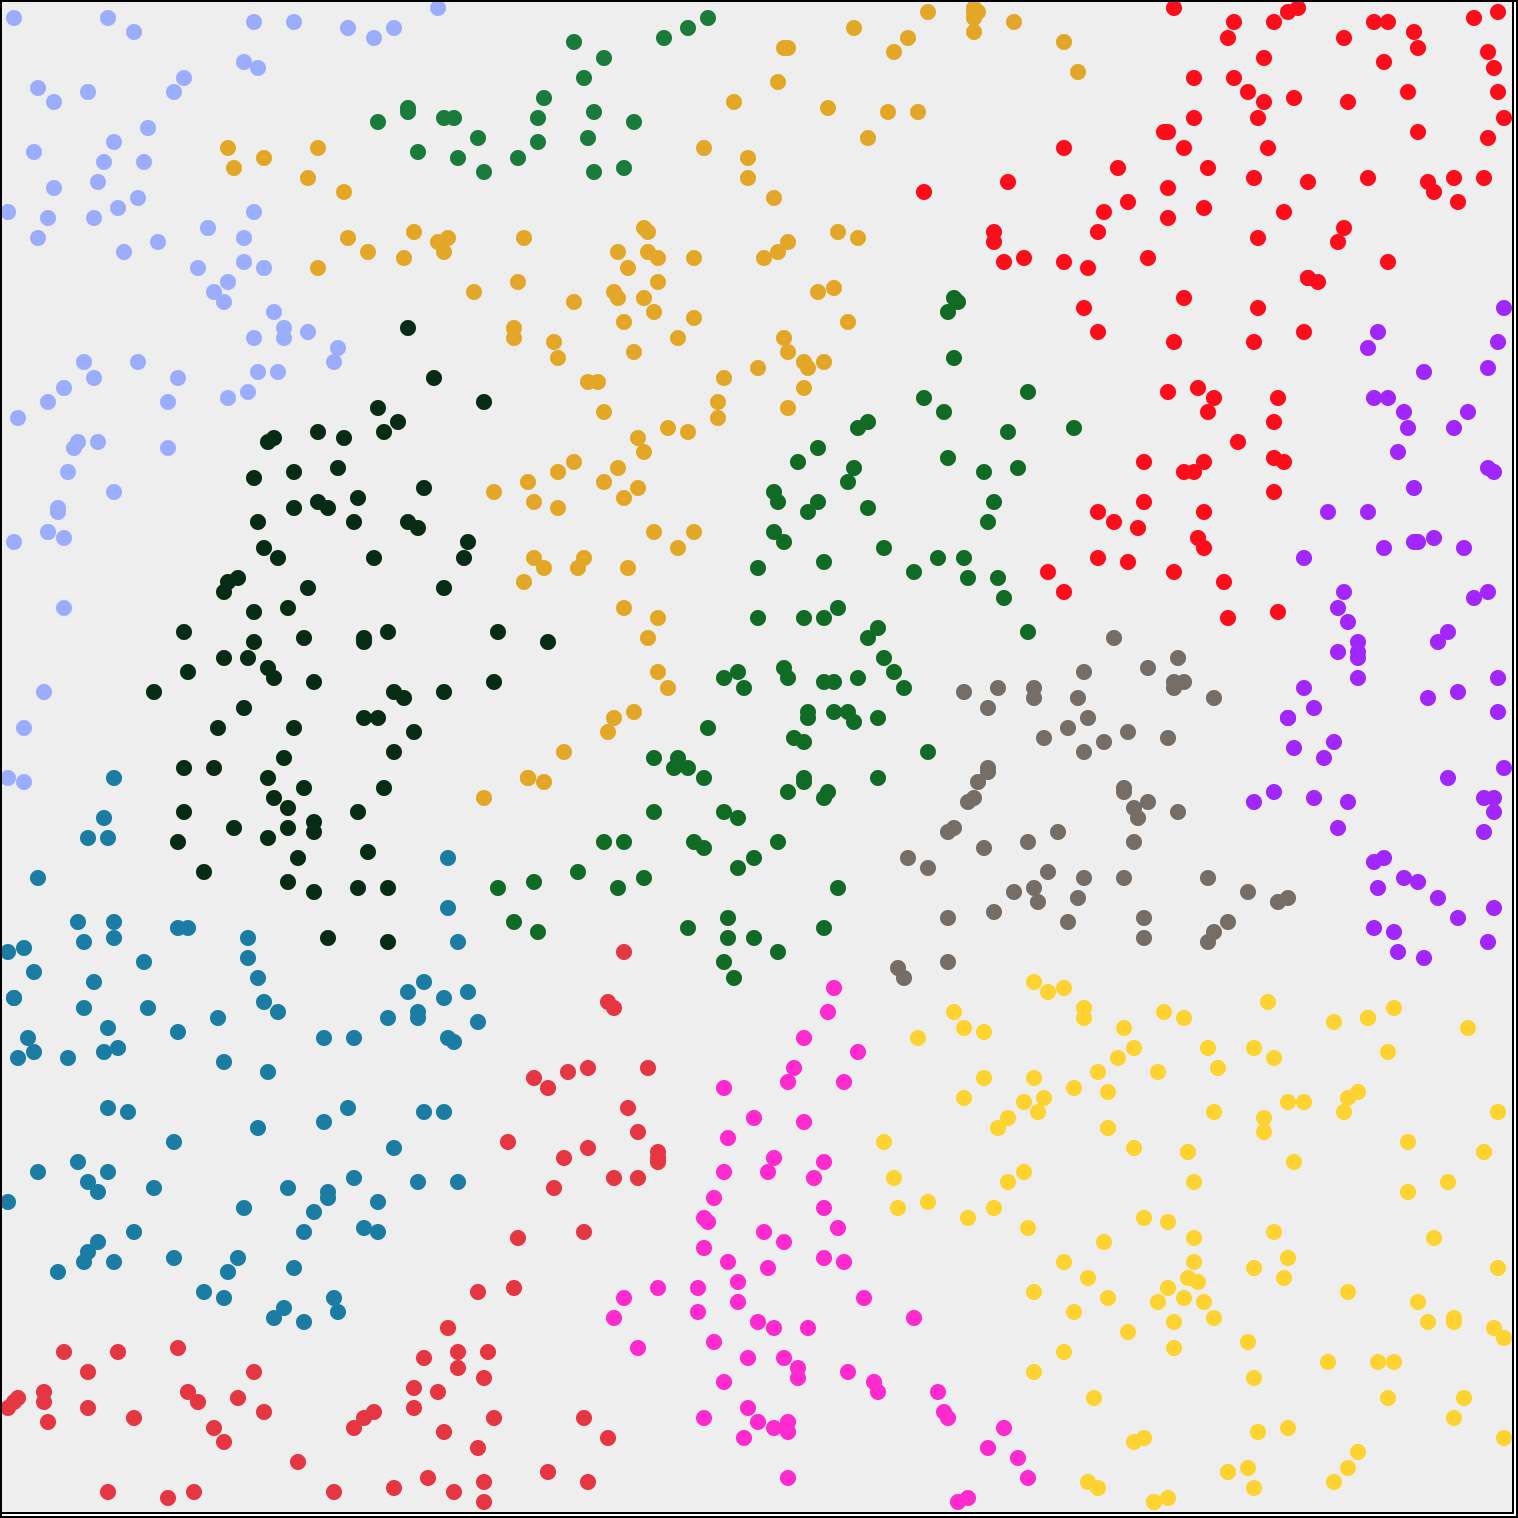
\includegraphics[width=6cm]{Images/computations/BASIC500x500_1000n.jpg} }}%
		\qquad
		\subfloat[Forks]{{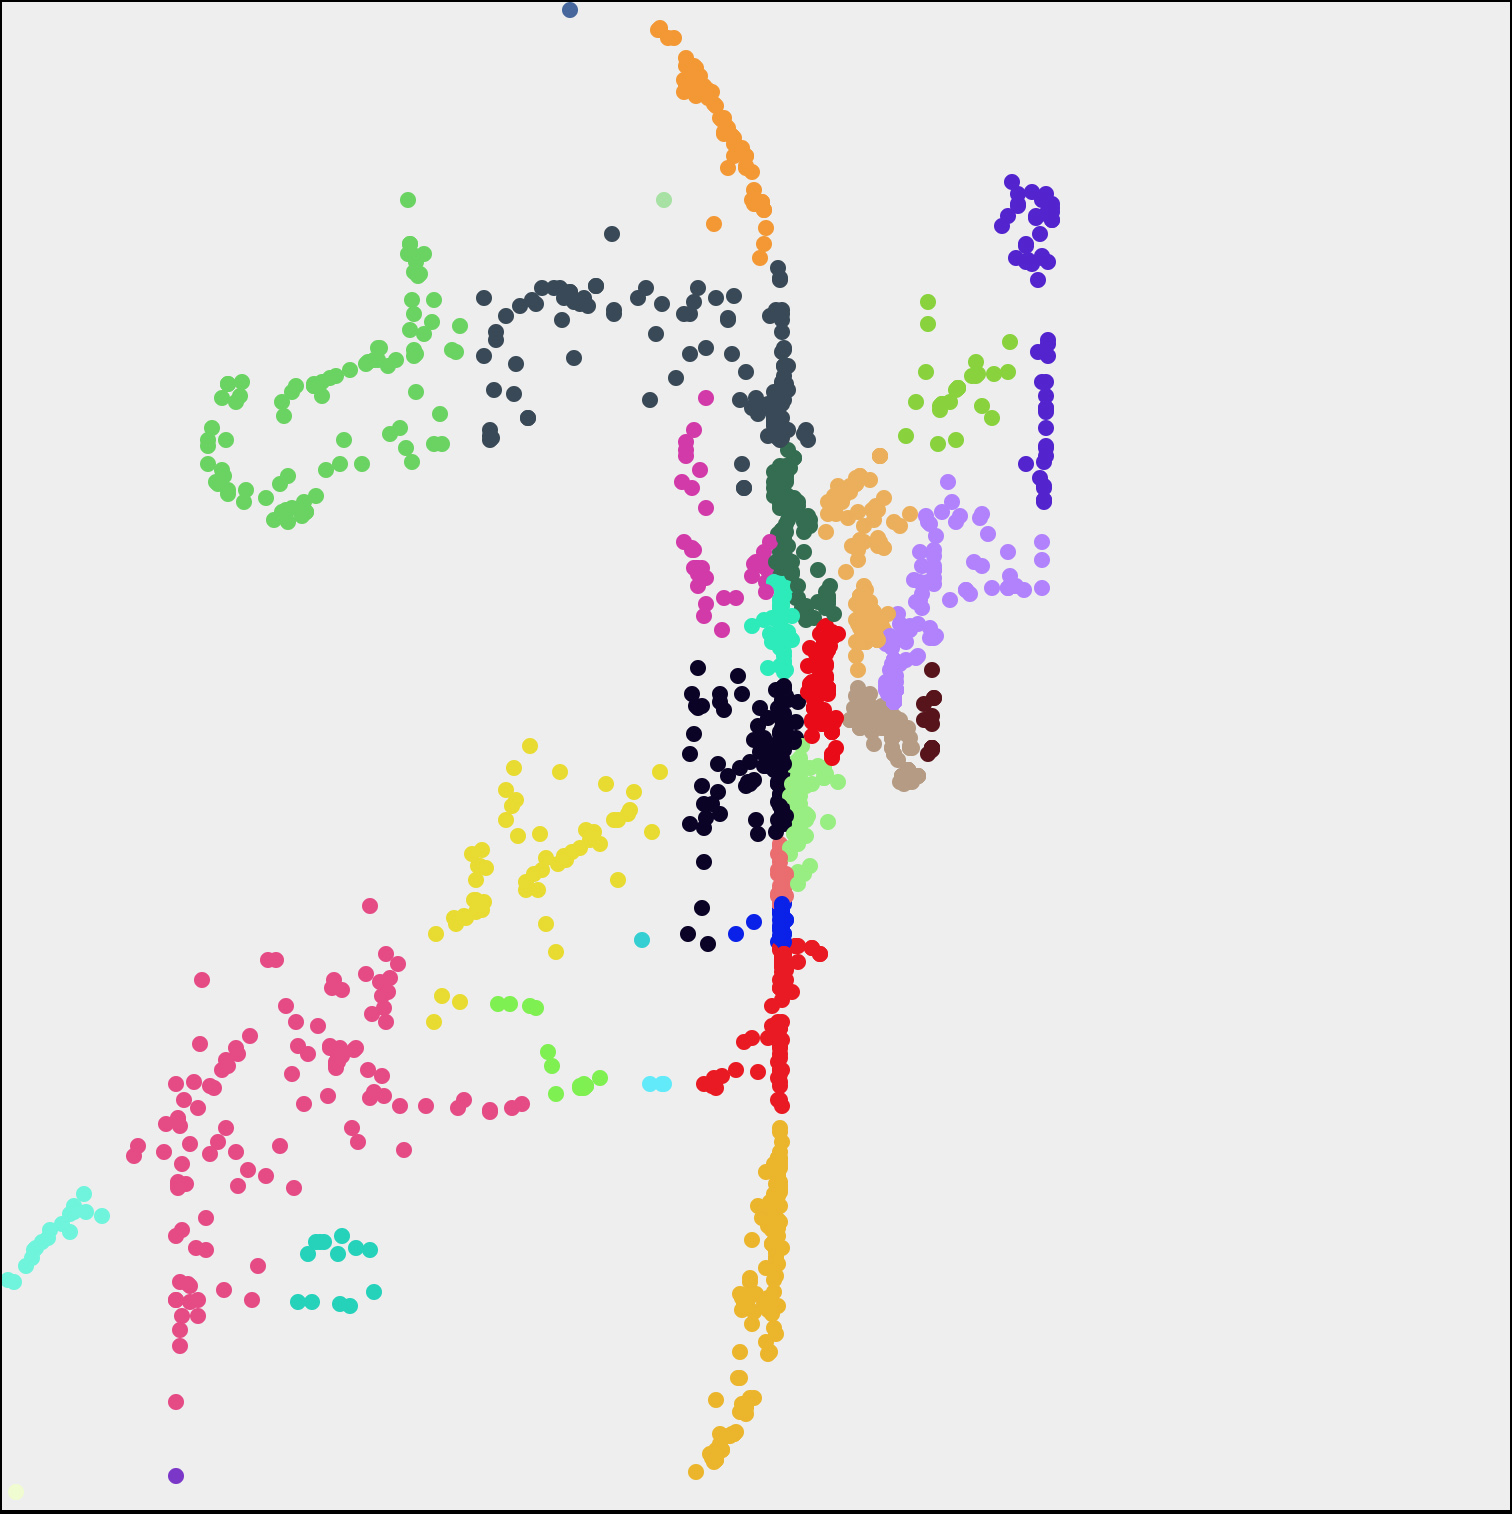
\includegraphics[width=6cm]{Images/computations/BASICForks.jpg} }}%
		\newline
		\subfloat[Lillehammer]{{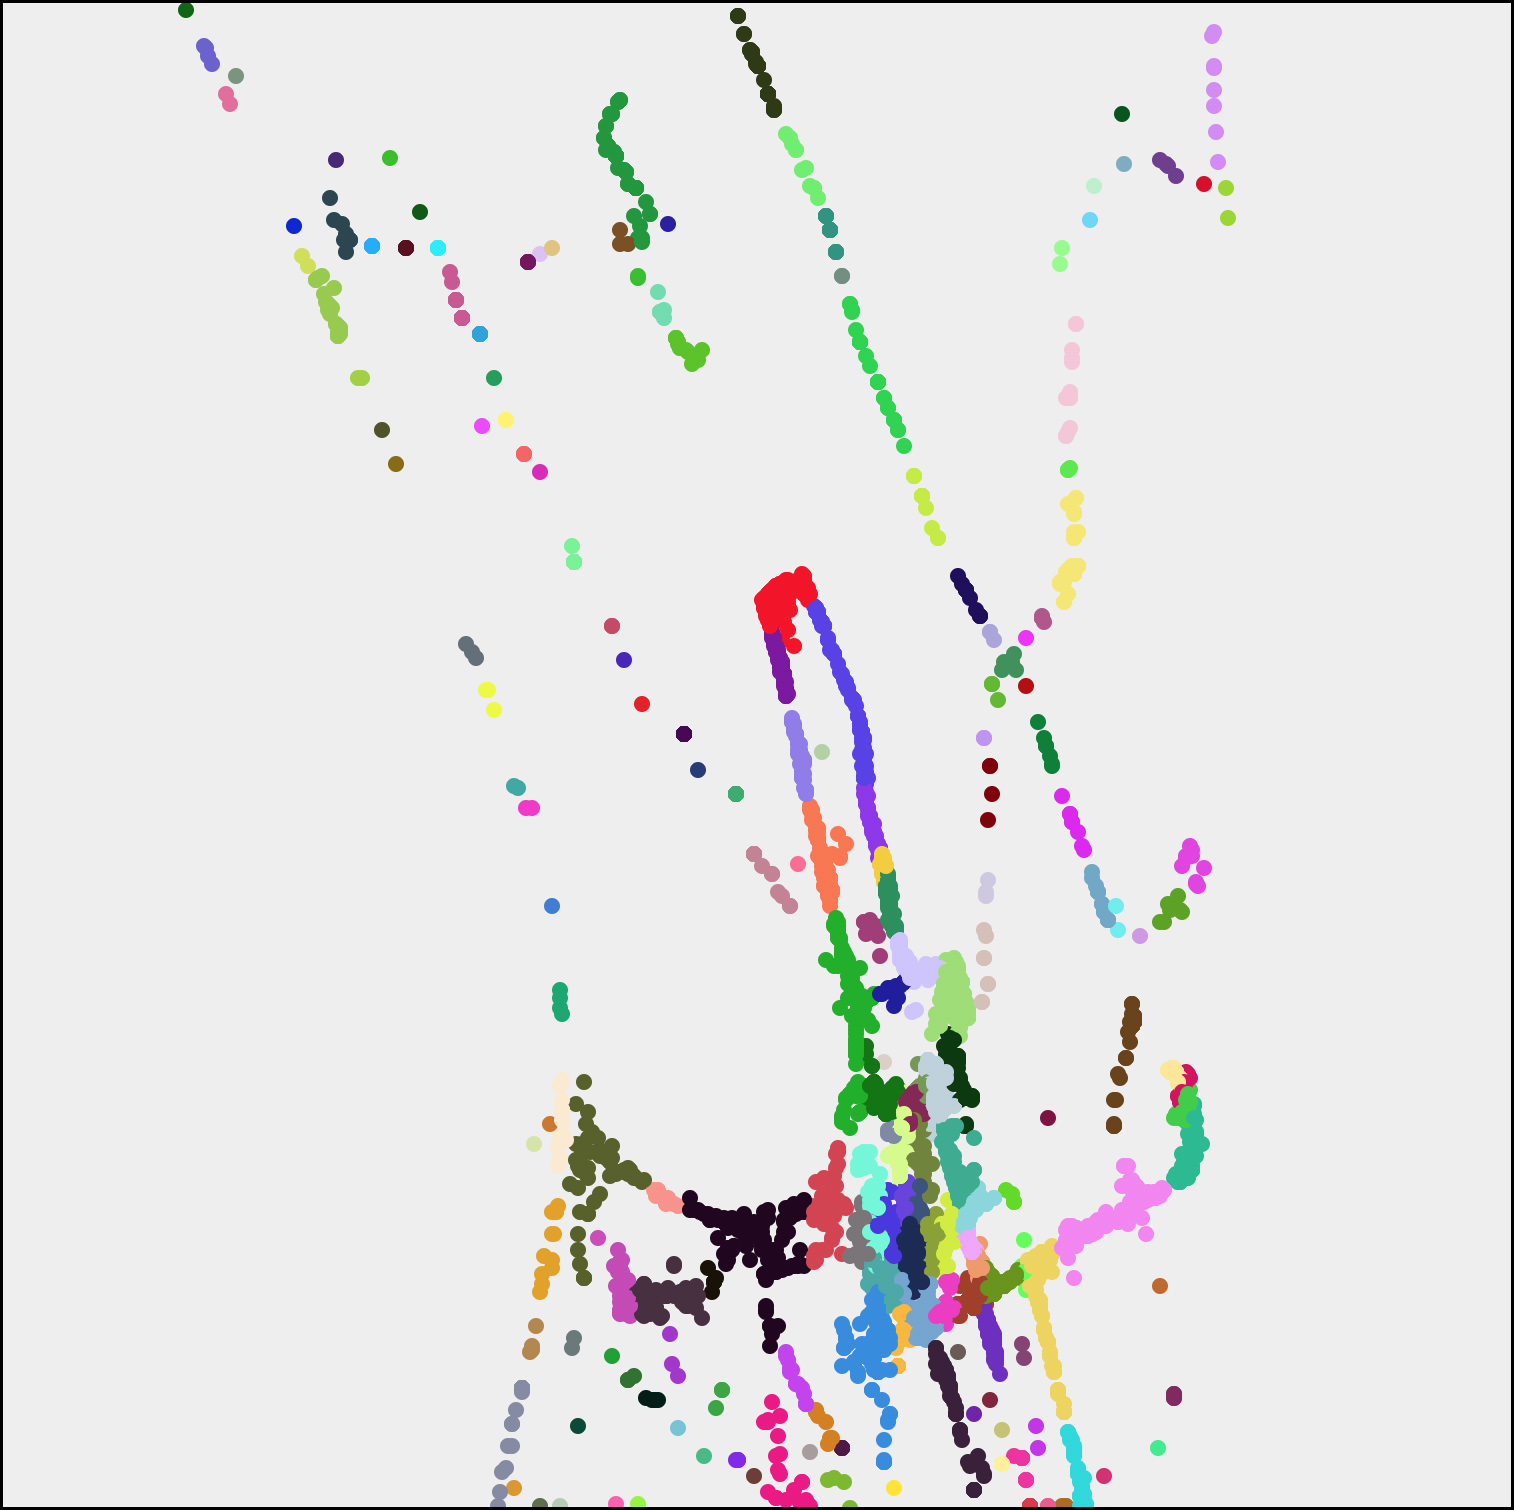
\includegraphics[width=6cm]{Images/computations/BASICLillehammer.jpg} }}%
		\qquad
		\subfloat[Tynset]{{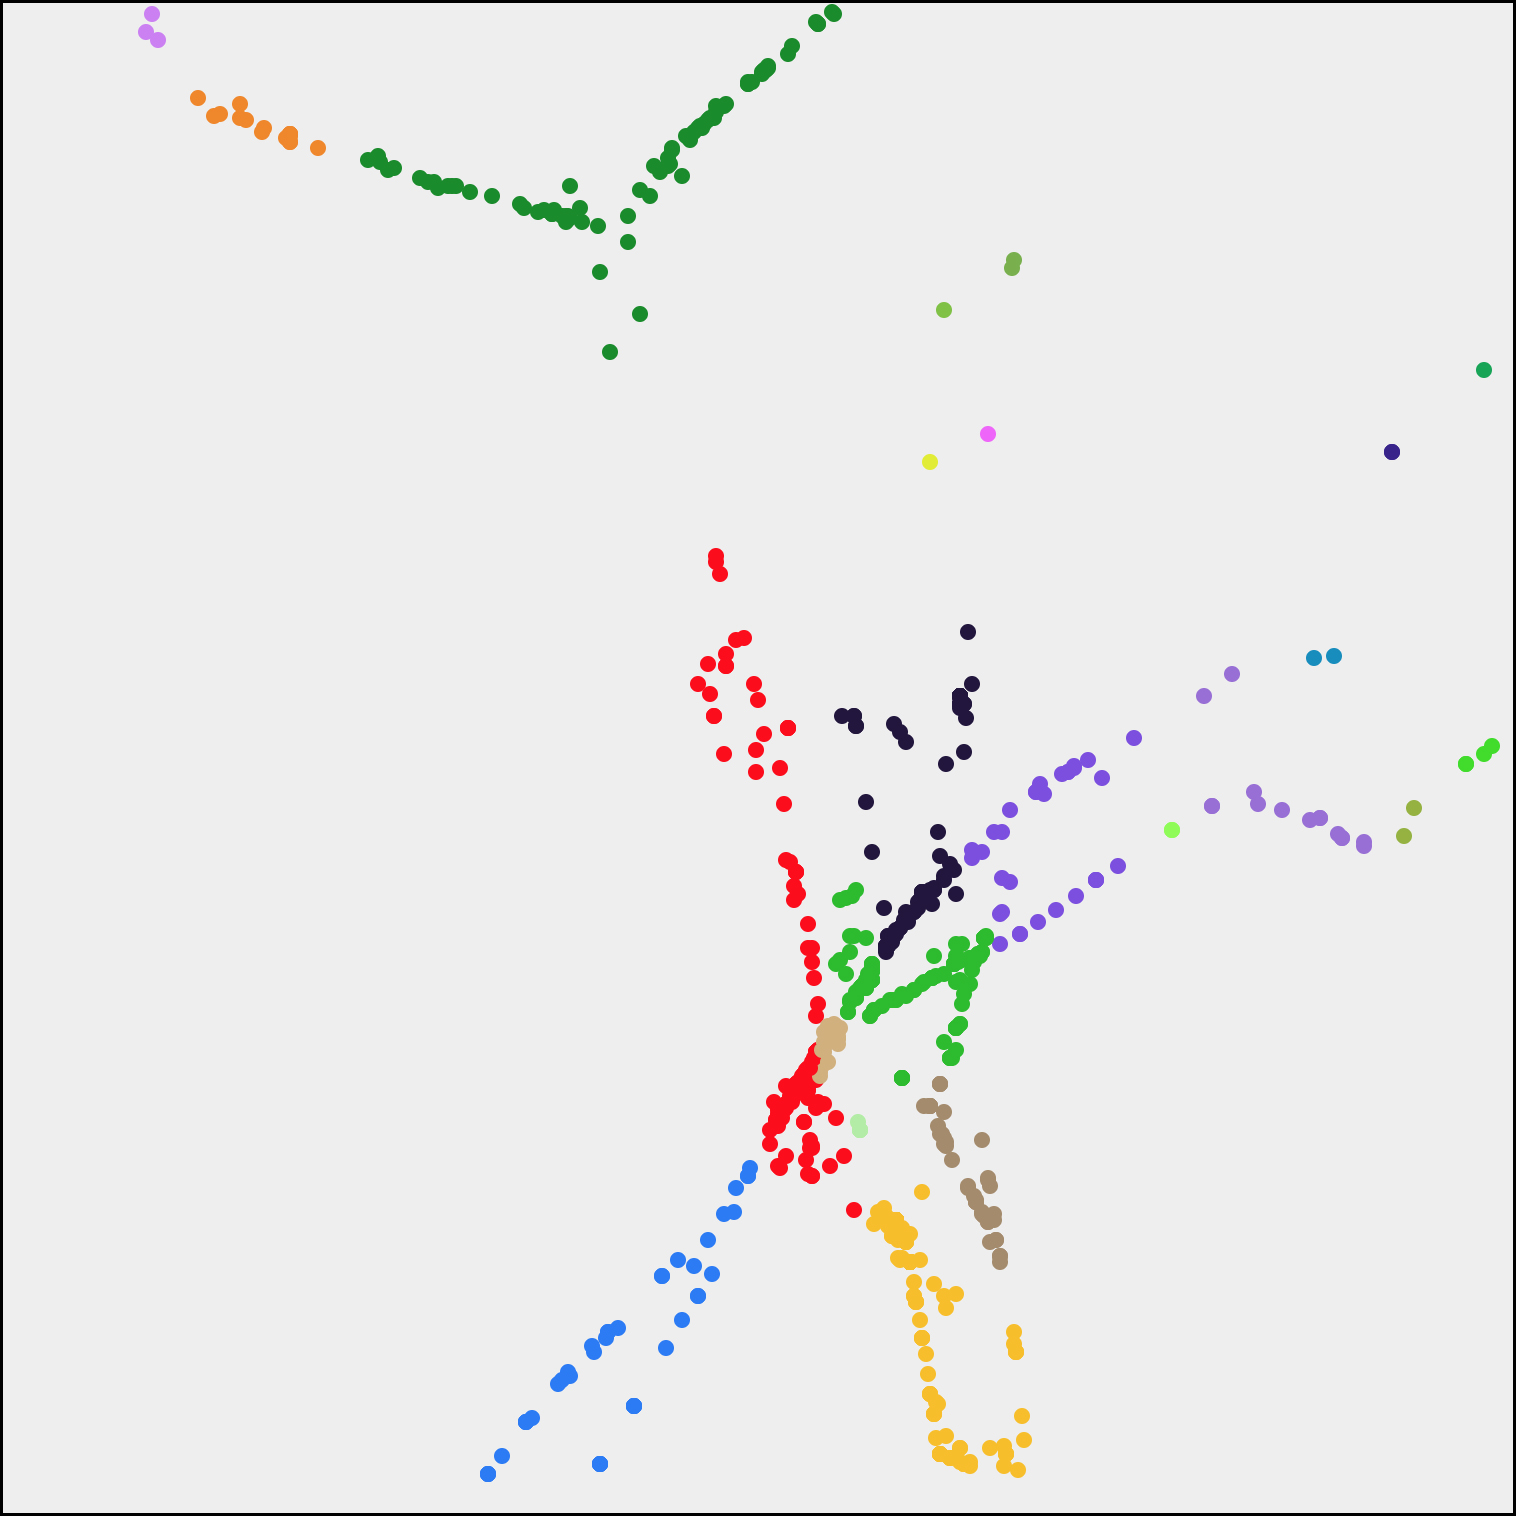
\includegraphics[width=6cm]{Images/computations/BASICTynset.jpg} }}%
		\caption{K-Nearest Neighbour Clustering on different topologies}%
		\label{fig:knearest}%
\end{figure}

%\begin{figure}[H]
%	\center
%	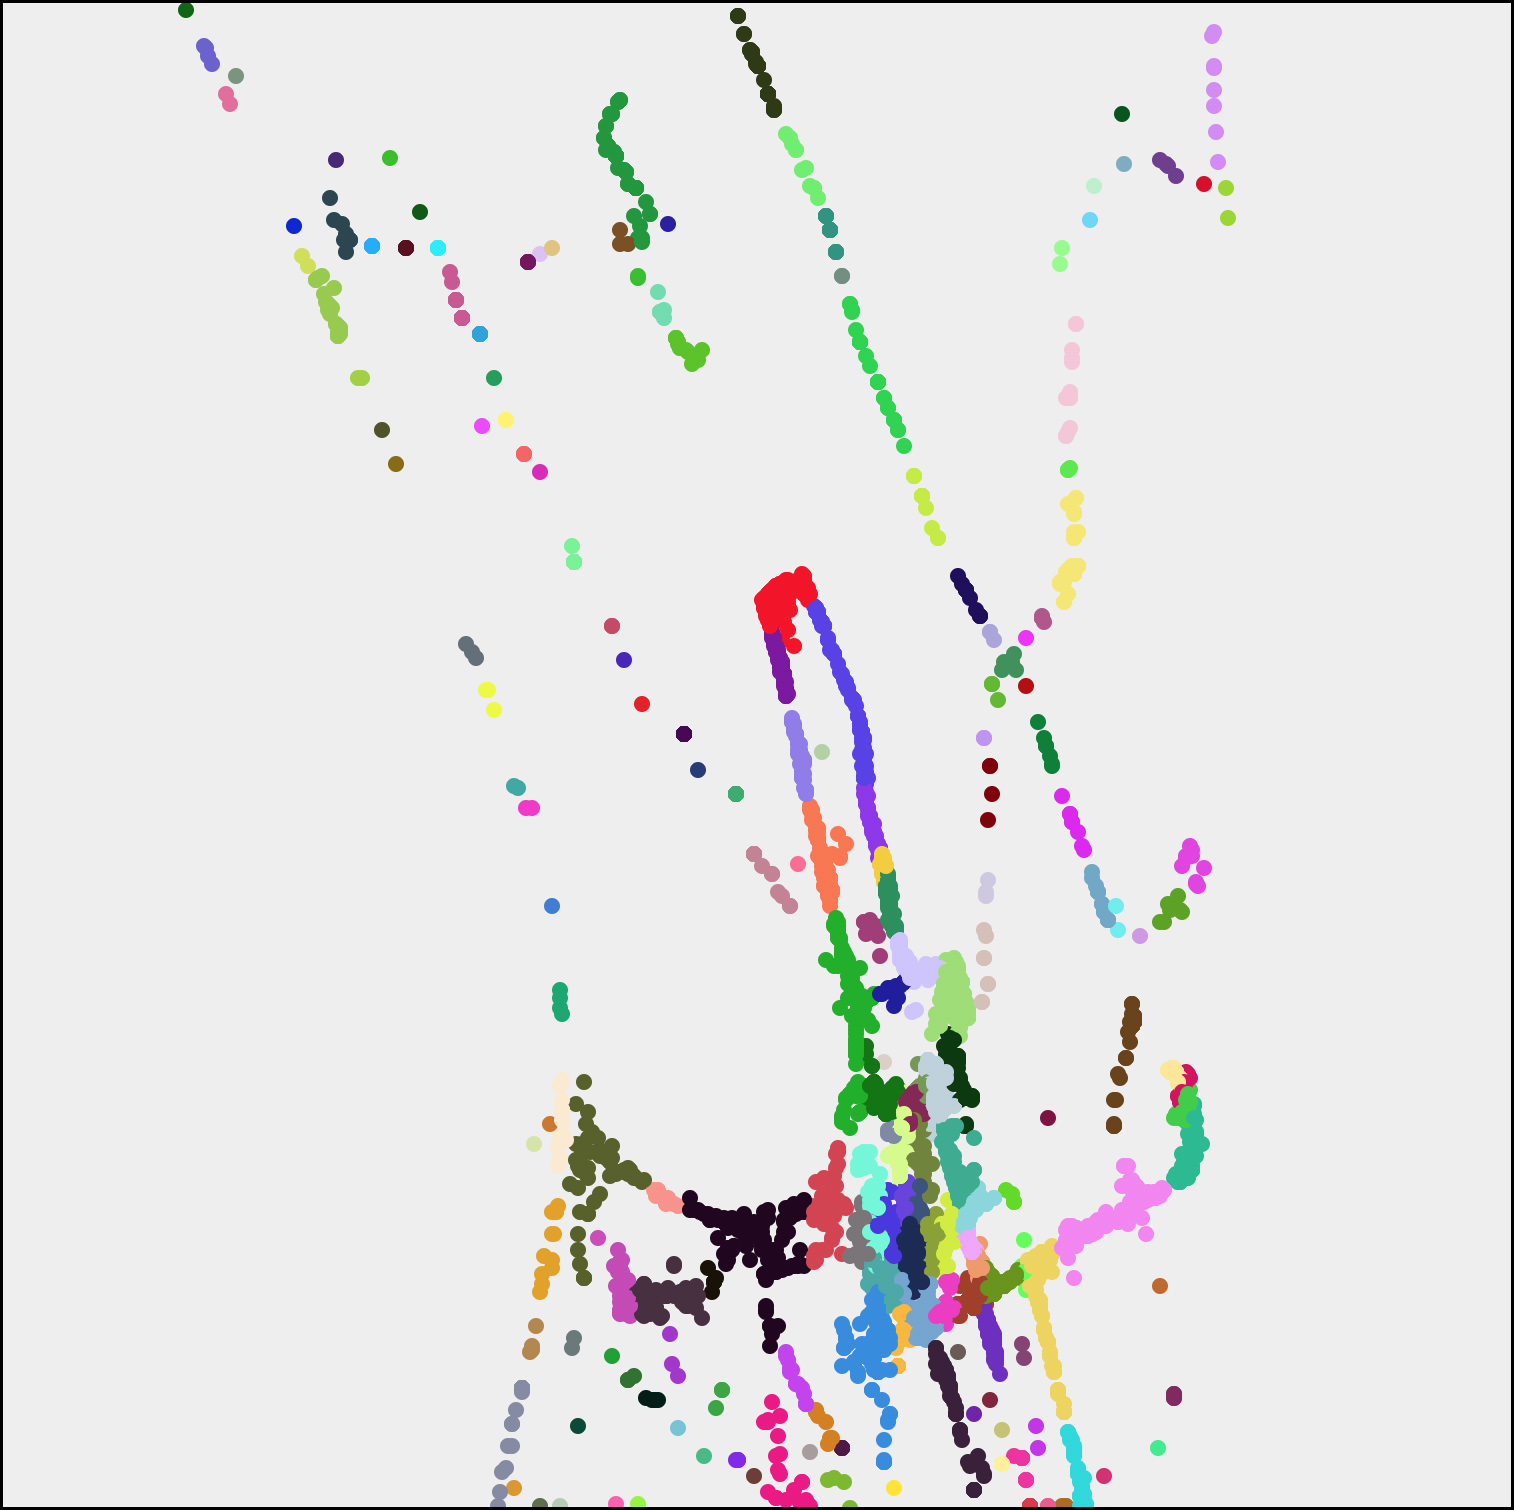
\includegraphics[scale=0.25]{Images/computations/BASICLillehammer.jpg}
%	\caption{K-Nearest Neighbour Clustering on nodes in Lillehammer, Norway}
%	\label{fig:basic_lillehammer}
%\end{figure}
%
%\begin{figure}[H]
%	\center
%	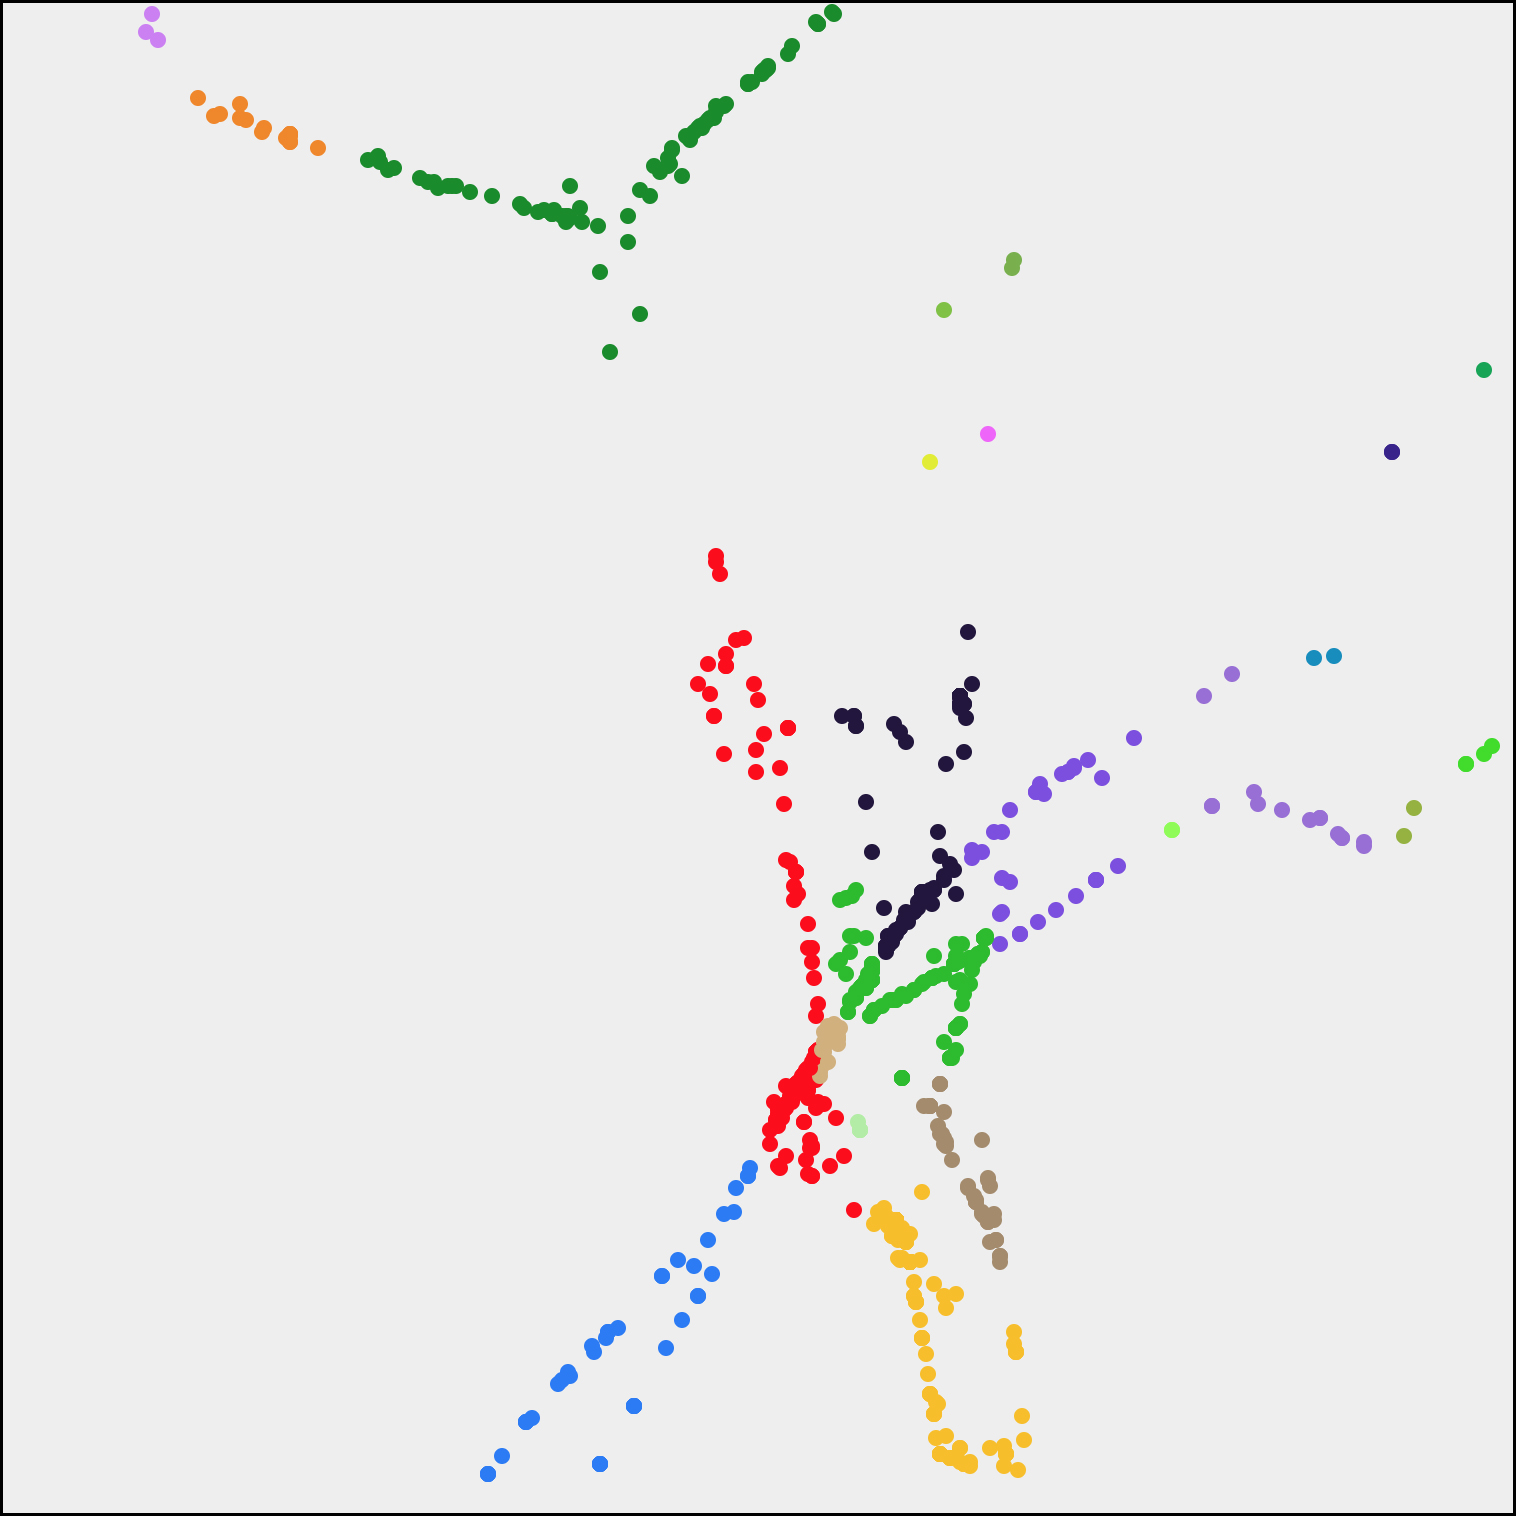
\includegraphics[scale=0.25]{Images/computations/BASICTynset.jpg}
%	\caption{K-Nearest Neighbour Clustering on nodes in Tynset, Norway}
%	\label{fig:basic_tynset}
%\end{figure}

\subsection{Evaluation}
By looking at the results of the simulations of the K-Nearest Neighbour Clustering it is obvious that clusters are created.  Even in the more chaotic topologies as Lillehammer,
there are distinct clusters that encompasses the closest nodes. However, there are two obvious problems with this algorithm:
\begin{itemize}
	\item In contrast to agglomerative clustering, our K-Nearest Neighbour Clustering algorithm does not care if the closest distance between the groups is pairwise mutual. This
		might lead to one group $a$ merging into another group $b$, even while $b$ has another neighbouring group $c$ that lies closer. If the maximum size K is reached during the merge of
		$a$ and $b$,  the resulting group will never be able to merge with $c$ even though that would have given a better cluster. 
	\item Once a cluster reaches the maximum size K, there is no possibilty for any other nodes to join the cluster.
		In our simulation of static topologies that might work, but in a real world scenario access points may turn on randomly, and be located in the middle of an already existing cluster.
		With the current algorithm there is no way to handle this event, and the node could not become a member of the cluster that surrounds it. 
\end{itemize}

In the next section we will look at how we can use group splitting to create a solution for these problems. 

%\subsubsection{Evaluation}
%The stength of this algorithm is its simplicity. Without using any special techniques it creates clusters that on first eyesight lookes quite promising. 
%An obvious weakness is that all nodes which are admitted to a group is never kicked out, no matter what happens during merges. This means that a very beneficial 
%merge can be discarded because of the large group size, even though many nodes in the group hardly disturbs anyone and should be deprioritized. 


%
%\begin{algorithm}[H]
%    \SetAlgoLined
%    \KwData{this text}
%    \KwResult{how to write algorithm with \LaTeX2e }
%    initialization\;
%    \While{not at end of this document}{
%	    read current\;
%	\eIf{understand}{
%		go to next section\;
%	    current section becomes this one\;
%    }{
%	    go back to the beginning of current section\;
%    }
%    }

%\caption{How to write algorithms}
%\end{algorithm}

\section{Introducing splitting}
To improve the K-Nearest Neighbour Clustering algorithm suggested in the previous chapter, we can introduce the notion of group splitting. By letting one cluster merge with another without knowing
if the merge is mutually beneficial, we are also accepting that not all merges will be optimal. A way to increase the chance of a group consisting of nodes that impacts each other severely
would be to accept merges that result in groups larger than K. The group would be too large, but also much more likely to be given the chance to merge with the nodes of highest impact. 
To reduce the group size back to K the least impactful nodes would have to be kicked out of the group, and this is what we call group splitting. 
This section is dedicated to two different suggestions of how a group could be split. 

\subsection{Introduction to K-means}
K-means is a clustering algorithm commonly used for classification purposes in machine learning, usually in the context of unsupervised learning. K-means
is an iterative algorithm designed to find a predefined amount of clusters in a data-set with unclassified data points. The amount of clusters to find is denoted by
K (hence K-means). 

K centroids are randomly placed somewhere in the data set, then the distance between each data point and each centroid is computed. All data points
closest to the same centroid becomes part of the same cluster set. When all data points are associated with a cluster, each cluster computes the mean position of all its data points.
The value of the mean position becomes the location of the new centroids. When all the new centroids are computed, one iteration is over. The algorithm continues until the position 
of all centroids remains unchanged after an iteration. When the position of the centroids are the same two iterations in a row, it means that the solution has converged and all K-clusters has been identified. 

A well known problem with K-means is that the result strongly depends on how the algorithm is initiatied. This problem can be reduced by running K-means several times
and choosing the best result of all the runs. 

\subsection{K-means splitting}
K-means clustering is not directly applicable to solve our clustering challenge. The reason we can not use K-means as the clustering algorithm is because the distributed nature of
the nodes and groups. Indeed, a vanilla implementation of K-means requires an extensive overview of the surrounding network topology. Our groups are limited to knowing about their members
and their neighbours. It would also be hard to choose a suitable K. Nontheless, K-means could still potentially help us create better groups. Let us consider the following.
We extend the K-Nearest Neighbour Clustering so groups are allowed to merge into a transient group if it exceeds the given maxsize.
The purpose of the large transient group is to identify the biggest gap between nodes, and split the group in two new groups with
$count(nodes) < maxsize$. If we set $K=2$, K-means can be used to identify where the transient group should be split to create two more connected clusters. 

Randomly picking two nodes to be centroids could lead to undesirable results where the two resulting groups are fundamentally different from the original ones.
Recall that what  we are trying to do is to reevaluate the divison line between the groups and see if K-means can achieve a better split. We can consider using the two negotiating nodes as centroids.
The negotiating nodes belong to different groups, and are the nodes that has observed eachother as the strongest interferer and are the nodes that are closest to the division lines between the group. If the distance between the most interfering nodes is lower after applying the K-means split, the new groups are applied.
On the other hand, if the distance is shorter (meaning a less optimal cut is found) the original groups are restored.
As the bootstrapped position of the centroids is planned and not random the result is deterministic and we don't have to run the algorithm more than one time to get the result. 
%



\subsection{Results}
\begin{figure}
	\centering
		\subfloat[Uniform]{{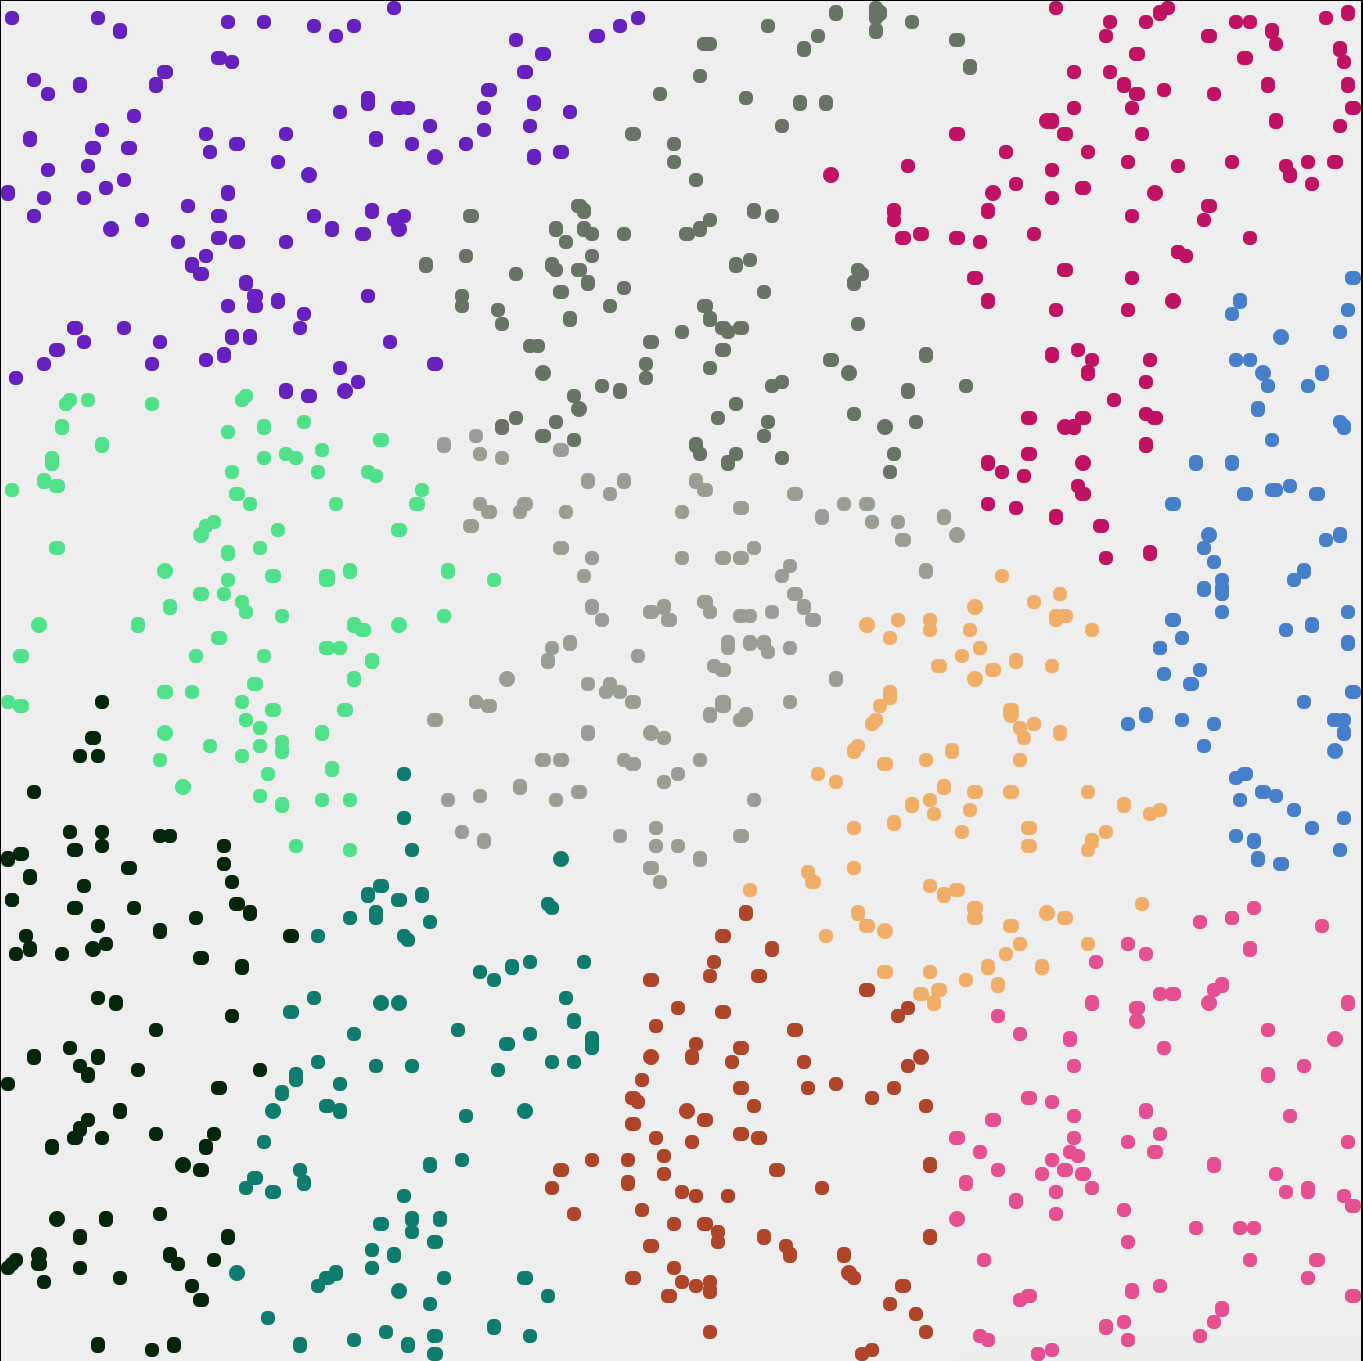
\includegraphics[width=6cm]{Images/computations/KMEANS500x500_1000n.jpg} }}%
		\qquad
		\subfloat[Forks]{{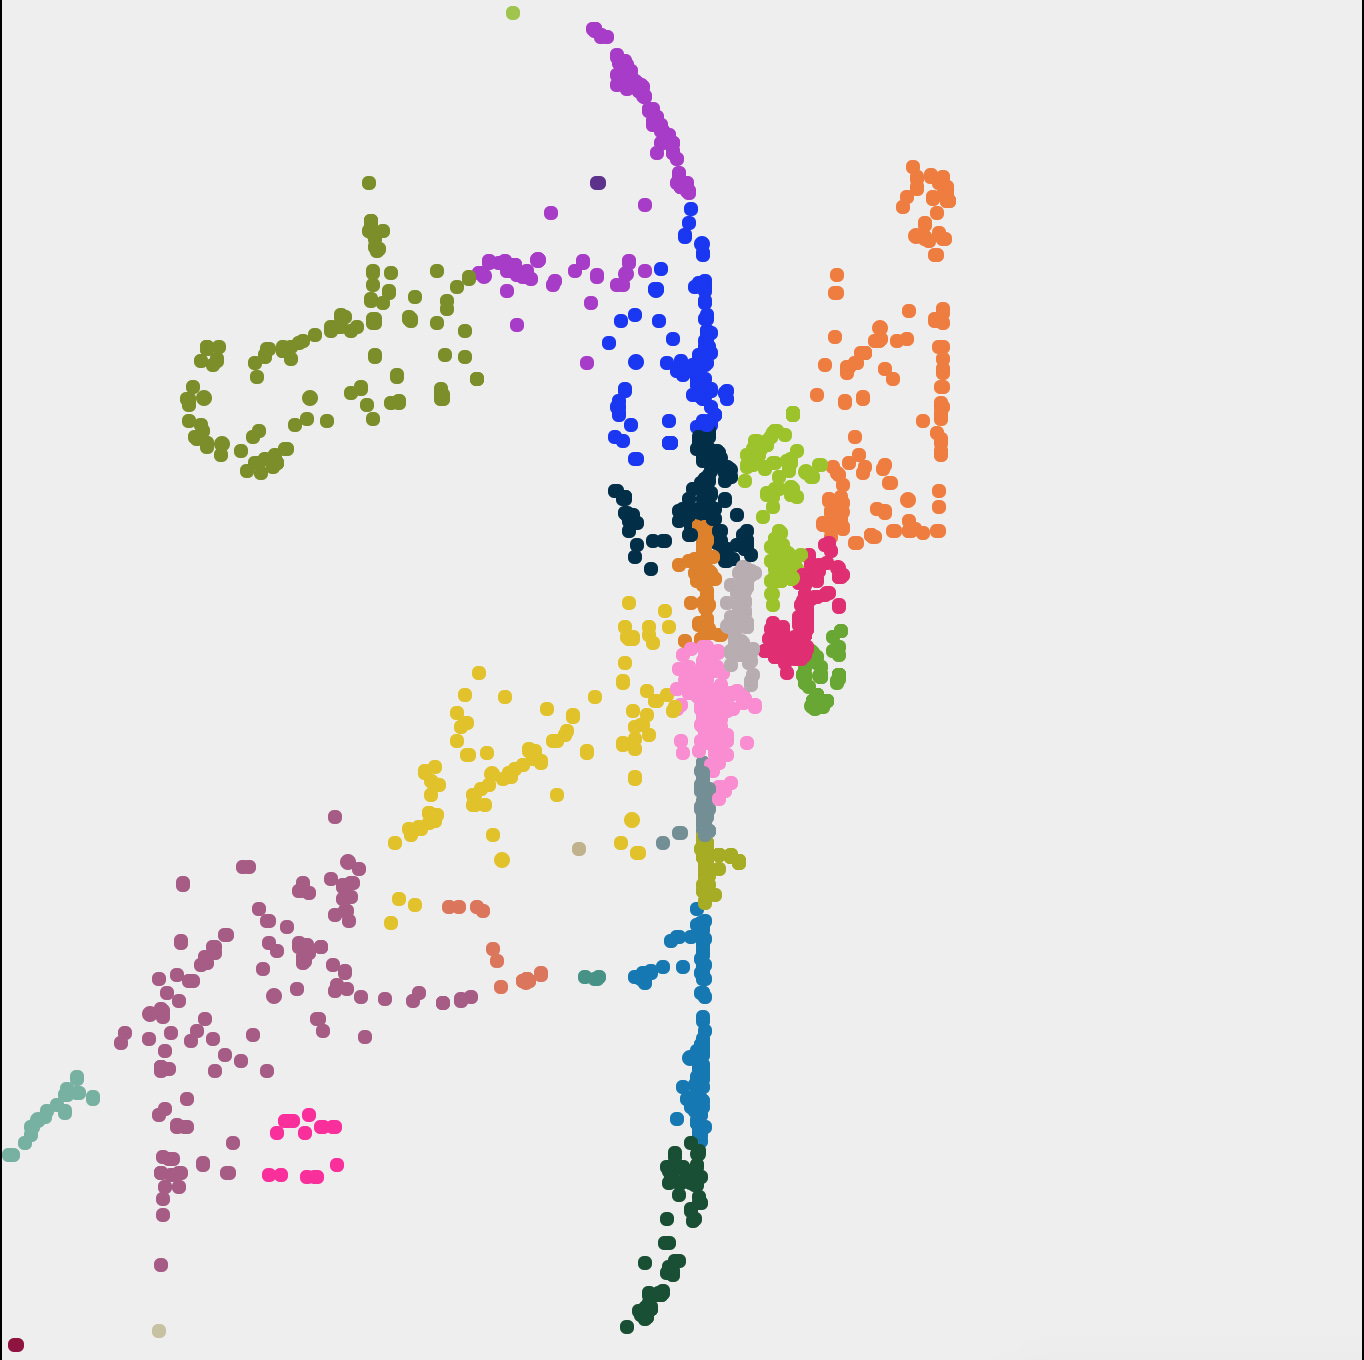
\includegraphics[width=6cm]{Images/computations/KMEANSForks.jpg} }}%
		\newline
		\subfloat[Lillehammer]{{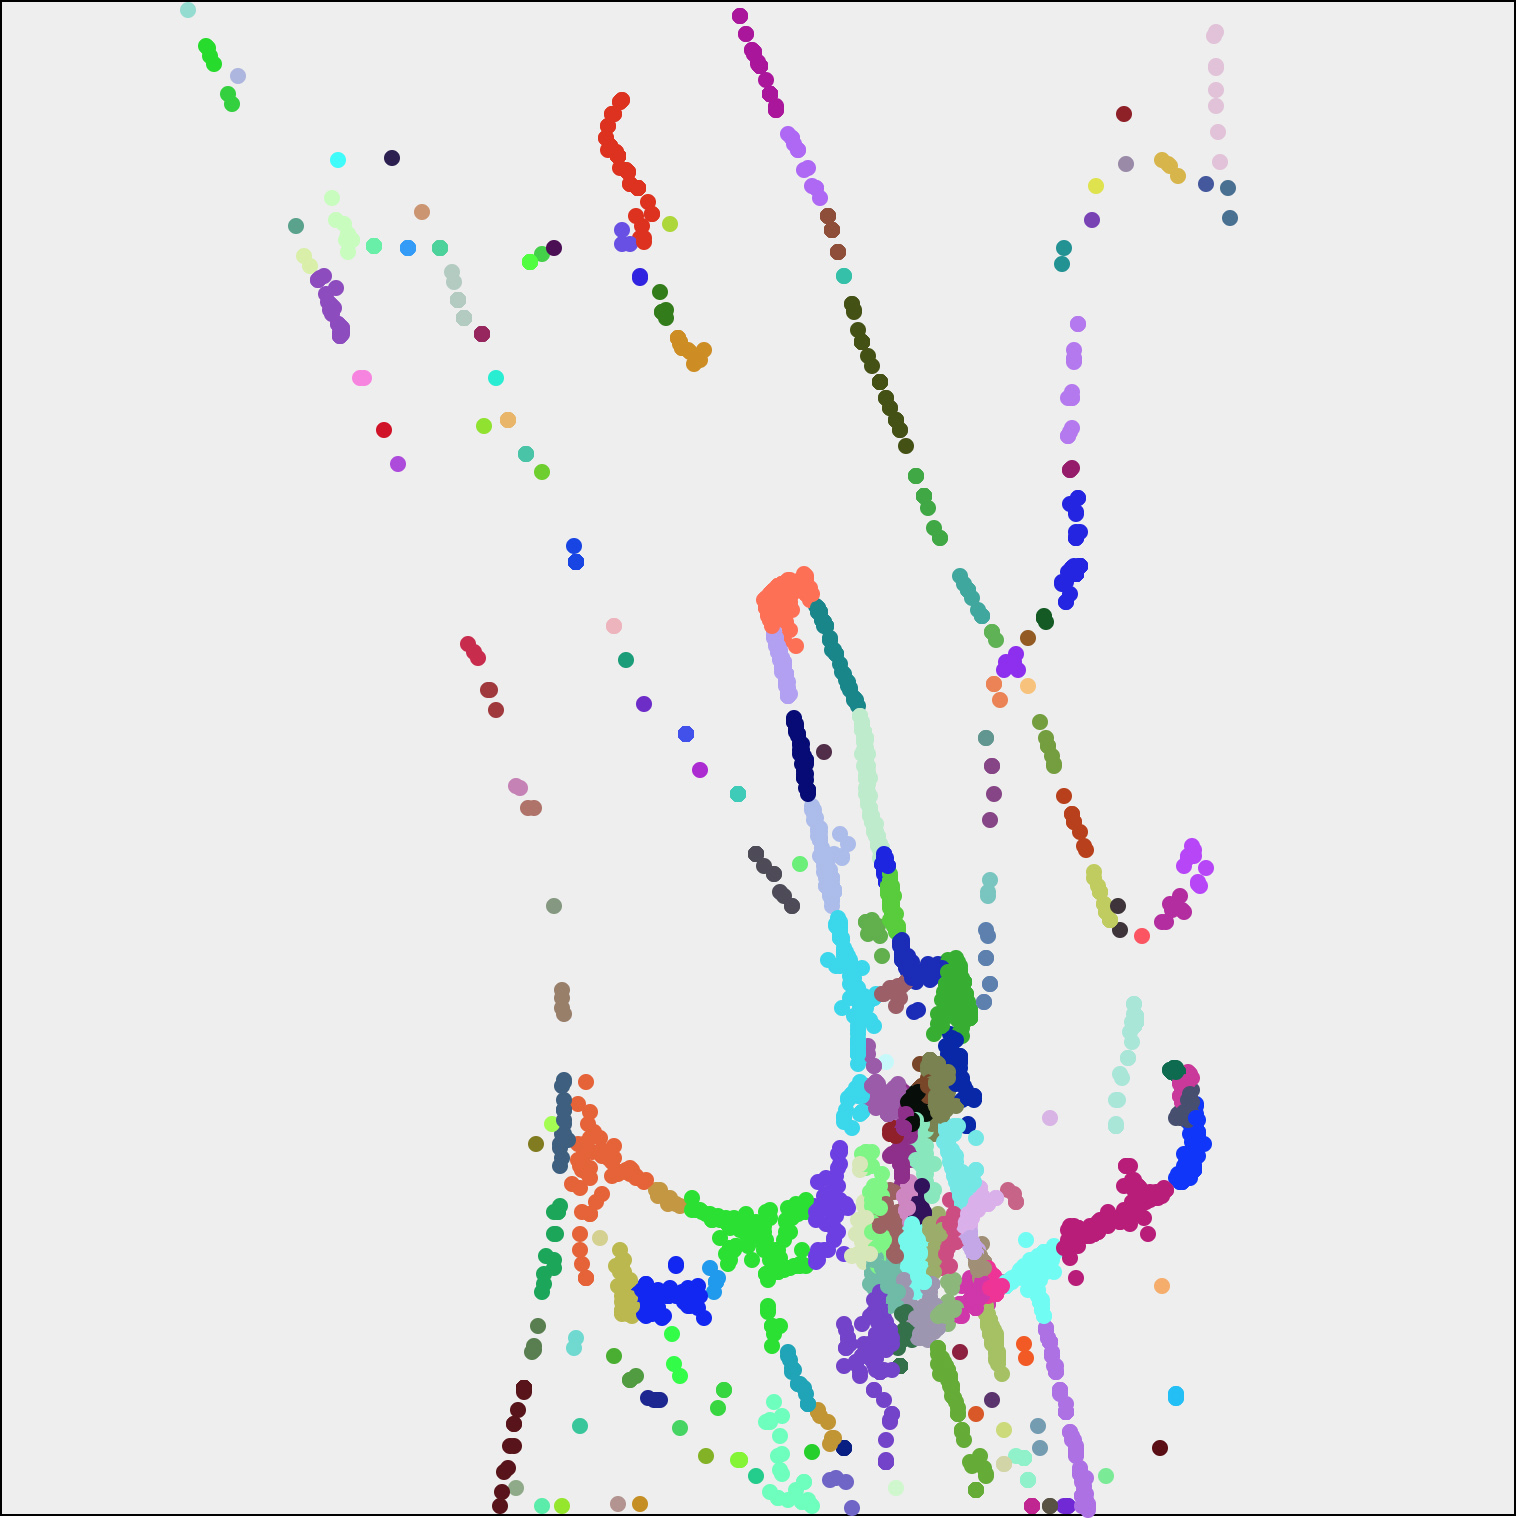
\includegraphics[width=6cm]{Images/computations/KMEANSLillehammer.jpg} }}%
		\qquad
		\subfloat[Tynset]{{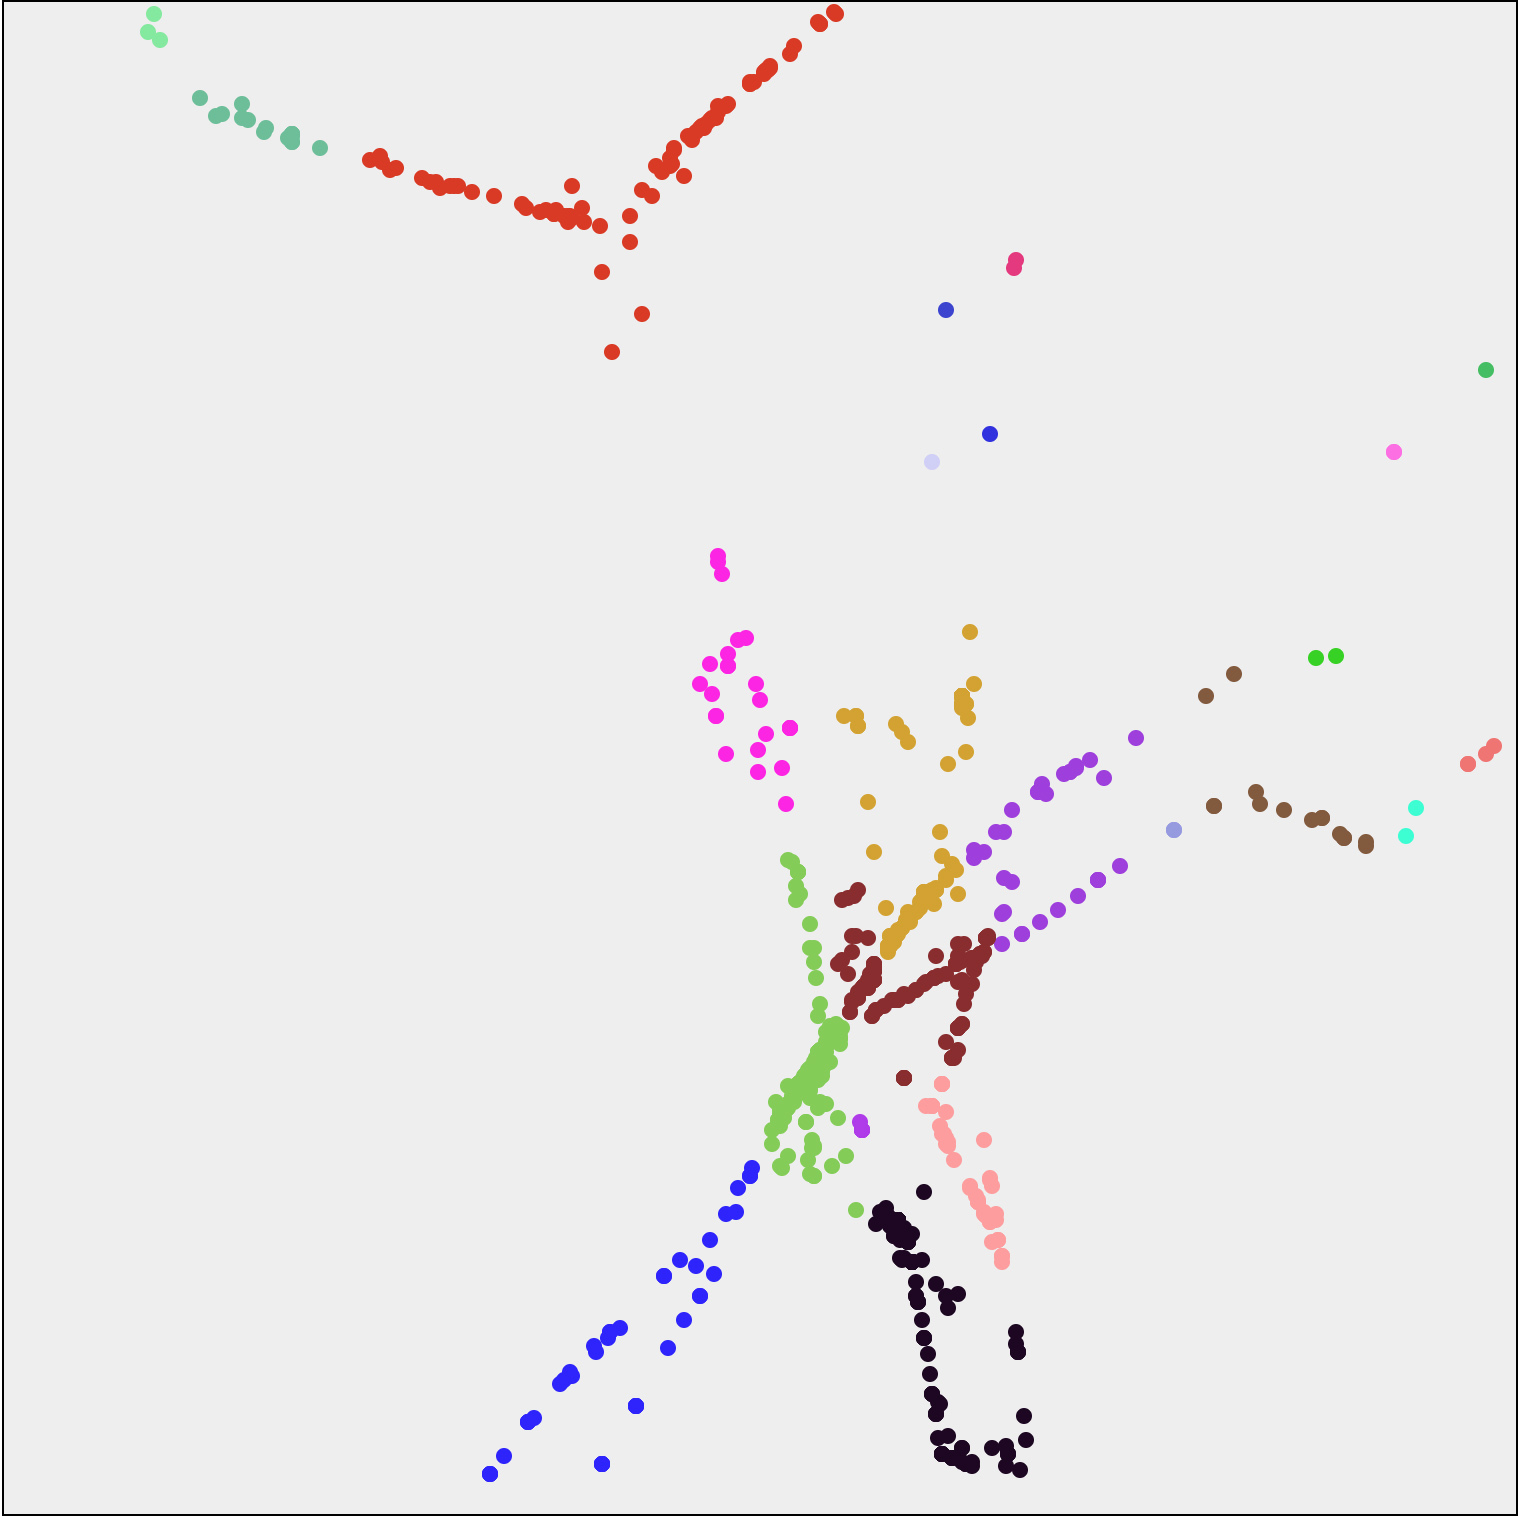
\includegraphics[width=6cm]{Images/computations/KMEANSTynset.jpg} }}%
		\caption{K-means splitting on different topologies}%
		\label{fig:knearest}%
\end{figure}







\subsubsection{Evaluation}

\subsection{Minimum Cut}

\section{Analysis}
\section{Evaluation program}

\subsection{Acquired knowledge}
\subsection{Weaknesses}
The computations have taught us about what kind of clustering could work with the assumptions we have set. Even so, there are several questions that still remains,
and without considering them we can not expect to get any concluding answers. 

\subsubsection{Dimensionality} 
Both the data we have created and the data fetched from \verb|wigle.net| takes the $x$ and $y$ axes in account. Obtaining data in three dimensions is harder.
Wigle positions the access points using longitude and latitude, and the simple reason for this is that all their data is based on ground-level triangulation.
As we are are only creating clusters based on information in two dimensions, we can not immediately assume that our results is applicable to 3-dimensional world. 
We could argue that it is resonable to think that a group creation algorithm that works well in two dimensions should also work well in three dimensions. Especially since our computations has only
used a virtual dBi value, and as we recall from the beginning this is a property calculated using the free space path loss formula. This formula takes only the distance between each node
as a variable. Nonetheless, other challenges may occur in 3 dimensions that we have not accounted for. For instance, 
the positioning of the nodes may we much denser than anticipated and its hard to estimate how that will impact the formation of groups. 

\subsubsection{Volatility} 
All the computations we have done takes a static network topology as an input. The static topology is an image of a network topology in a given state, and is not representative
of the volatile nature of modern networks. While it is true that most access points are relatively stationary and constant, it is increasingly popular to create
ad-hoc on-demand Wi-Fi networks using cell phones or a computers as access points. Additionally resetting of routers, power outages, etc. means that access points come and go. 
Hence it is indisputable that network topologies are volatile, and the group clustering algorithm should, when final, run as a continous operation. 

\subsubsection{Computed interference vs observed interference}
Our group computations has been based on the RSSI of all nearby access points, and the dBi values that denotes all RSSIs were calculated using the free space path loss formula.
As distance is the only variable that affects the result of our RSSI calculation, it means that all RSSI levels forms a symmetric binary relation between nodes. In the real world 
this is not the case. Access points may interfere with each other differently, and the RSSI values may change when there are variations in the environment. We have assumed
that there is always another access point that disturbs the most. If the RSSI values changes rapidly, so may also the access point that disturbs the most. 

%\subsection{Uniformly distributed nodes}
%We will look at how groups were created in different topology scenarios. 
%All topologies presented in this section was created by the topology generation program,
%but with different input parameters. Groups are distinguished by node color, where nodes
%of the same color represents members of the same group. 
%%\subsubsection{Scenario 1}
%Computed with 200 nodes with a maximum of 128 members in each group.
%
%As can be seen in figure \ref{fig:200_128} the algorithm divides the nodes in two
%sections. For clarity, a divisive line has been drawn around each group,
%in case colors are not available.
%When two major groups merged, the biggest groups surpasssed 128 members and began
%kicking out members. The excess members formed the black group at the bottom. 
%
%\begin{figure}
%\center
%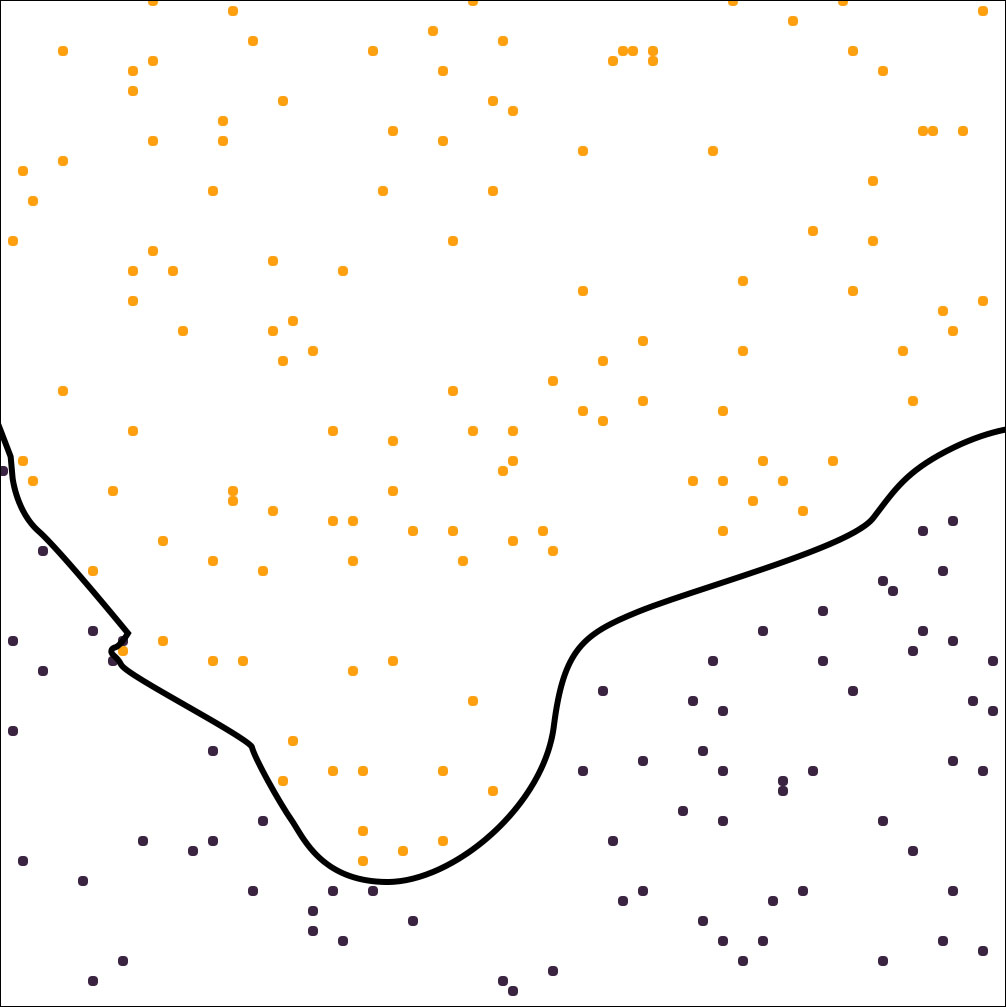
\includegraphics[scale=0.45]{Images/grouptest_1.jpg}
%\caption{200 nodes, $memberThresh=128$, $size=200x200$}
%\label{fig:200_128}
%\end{figure}
%
%
%\subsubsection{Scenario 2} \label{scen2}
%Computed with 200 nodes with a maximum of 10 members in each group.
%
%The result of this computation, seen in figure \ref{fig:200_10}, is a little less obvious.
%The groups are again distinguished by different color, but for clarity we add a gray connecting
%blob for nodes in the same group. Also blobs connected with a line are in the same group. 
%
%It is worthy to take notice that one group is especially scattered around the graph.
%At first eyesight, it looks like an algorithm deficiency, but the reason is quite simple:
%when nodes are kicked out of a group during a merge, they will connet to other nodes
%that belong in a group where $n$ has not yet reached $memberThresh$. When this have happened a couple of times, everyone has found a group except for the remaining few.
%These are typically straggler nodes or smaller clusters separated from the others.
%They are not big enough to reach the group $memberThresh$ on their own, so the merge with other
%nodes that are in unmaxed groups. Thus, even though they have neighbours which
%influence them more, they can only merge with nodes further away,
%because that is the only unlocked group that remains.
%\begin{figure}
%\center
%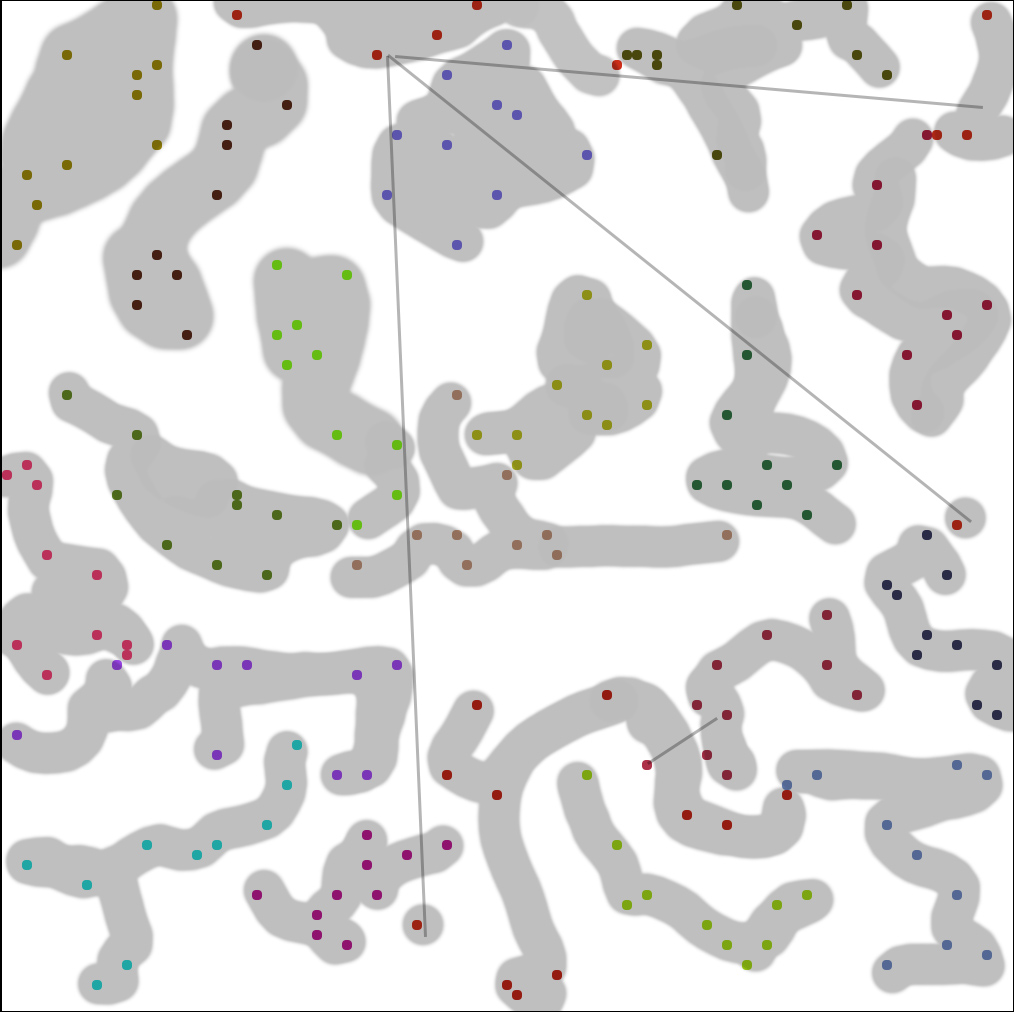
\includegraphics[scale=0.45]{Images/grouptest_2.jpg}
%\caption{200 nodes, $memberThresh=10$, $size=200x200$}
%\label{fig:200_10}
%\end{figure}
%
%\subsubsection{Scenario 3}
%Computed with 5000 nodes, with a maximum for 64 members in each group. 
%
%Figure \ref{fig:2000_64} shows the result of the computation. Because of the quantity
%of nodes and the clear separation of groups, they are easily distinguished by color.
%This topology is much denser than the others, and can vaguely resemble the density of highly populated areas.
%
%We can clearly see that the overall tendency is that groups are formed
%in concentrated areas of nodes. However, some groups are scattered, sometimes
%all over the map. An example of a scattered group is highlighted
%in figure \ref{fig:2000_64}. Its  member nodes has a thicker black line around them. 
%\begin{figure}
%\center
%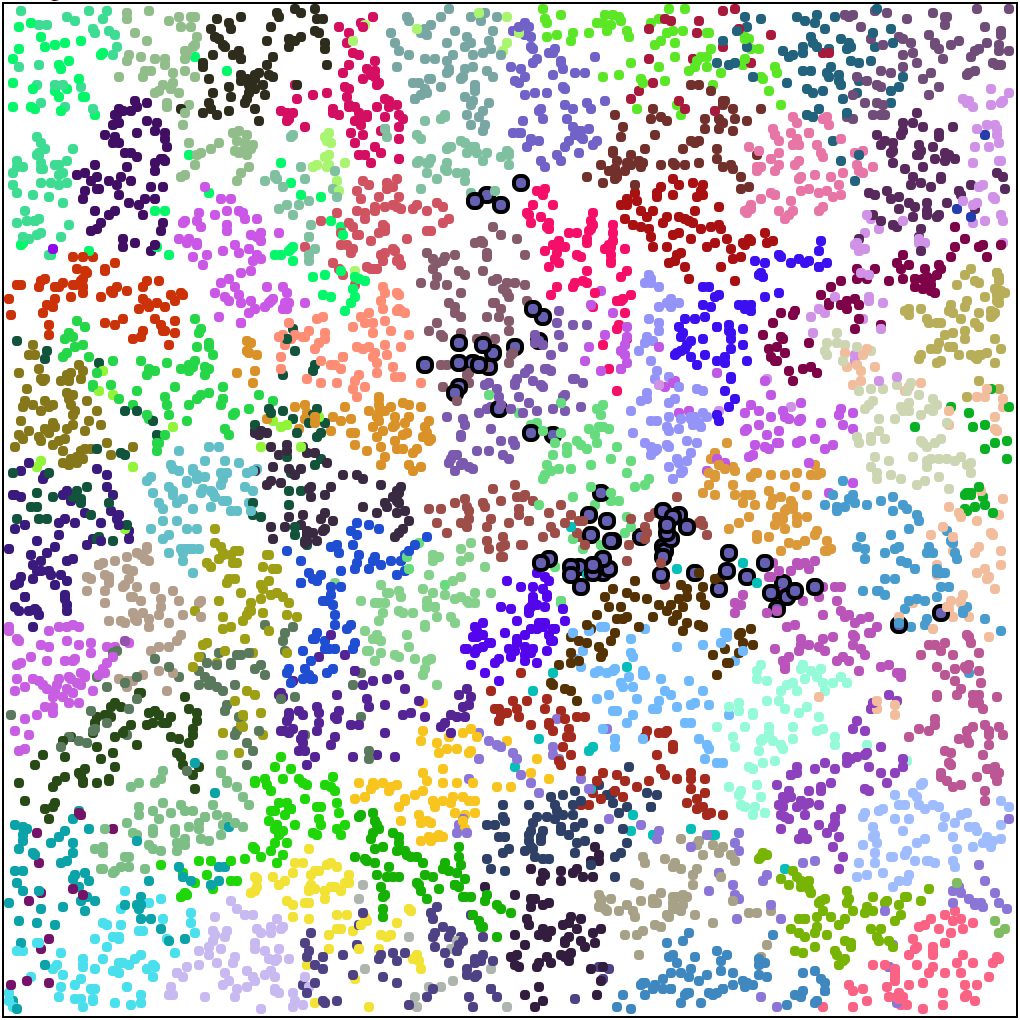
\includegraphics[scale=0.45]{Images/scenario3alt.png}
%\caption{5000 nodes, $memberThresh=64$, $size=2000x2000$}
%\label{fig:2000_64}
%\end{figure}






%
%\begin{figure}
%\centering
%\begin{minipage}{.6\textwidth}
%	\center
%	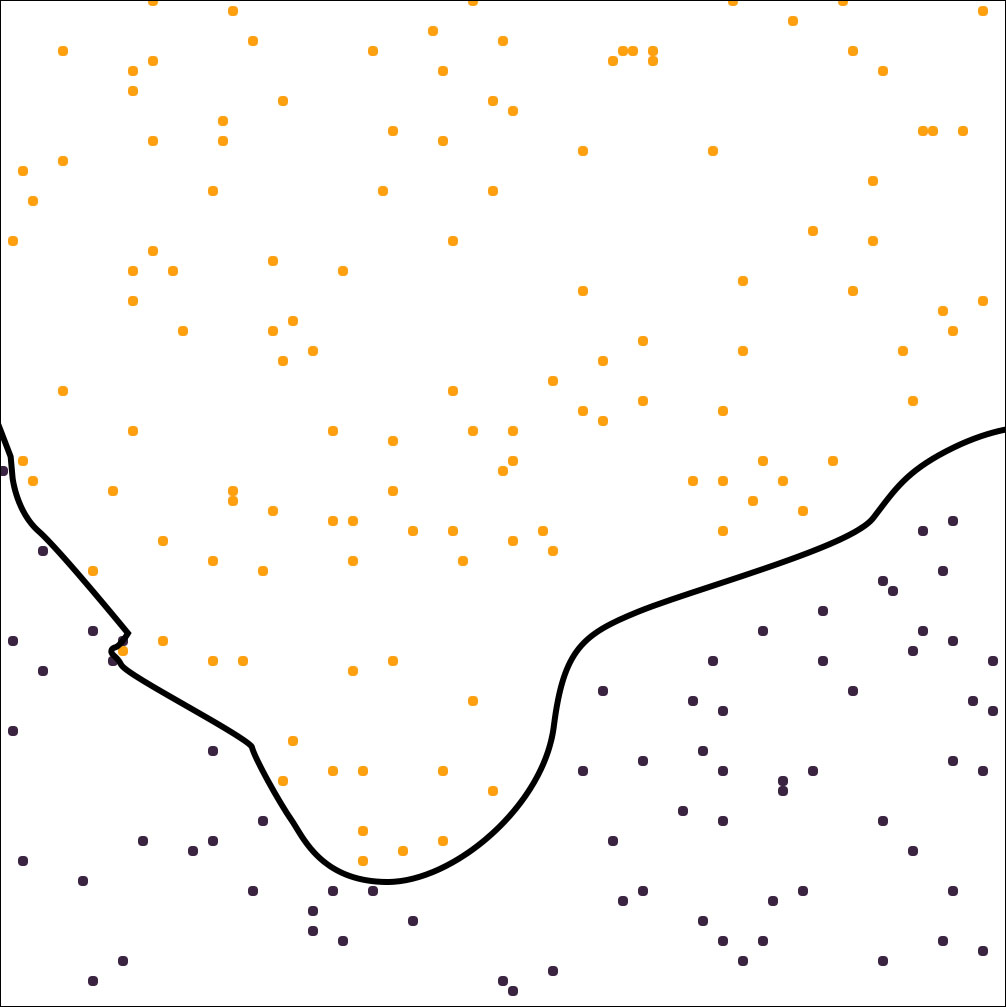
\includegraphics[width=0.9\linewidth]{Images/grouptest_1.jpg}
%	\captionof{figure}{\newline200 nodes, $memberThresh=128$}
%	\label{fig:200_128}
%\end{minipage}%
%\begin{minipage}{.6\textwidth}
%	\center
%	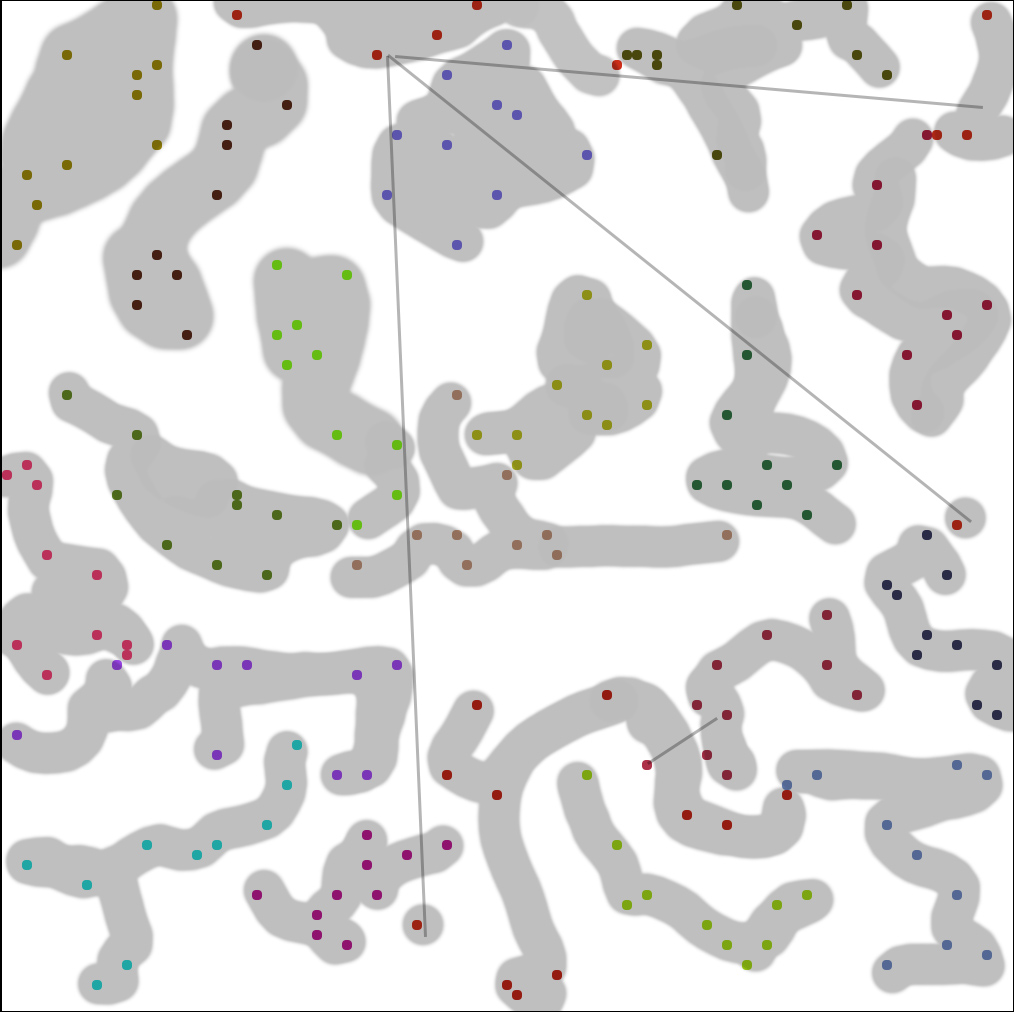
\includegraphics[width=0.9\linewidth]{Images/grouptest_2.jpg}
%	\captionof{figure}{Another figure}
%	\label{fig:test2}
%\end{minipage}
%\end{figure}



%
%\section{Results}
%By running the scripts that parses data from Wigle on populated areas, we should get an idea 
%on how the algorithm performs in more realistic topologies. We will have a look at three
%scenarios where the group allocation data is based on AP-data. 
%
%Three suitable locations has been selected to perform the testing on Lillehammer (Norway)
%a smaller city, Tynset (Norway) a less densely populated area, 
%and Forks (Washington, United States). All tests were 
%ran with a maximum group size of 128, and a $-dBi$ threshold of $-80$. 
%
%\subsubsection{Lillehammer}
%\begin{figure}
%\center
%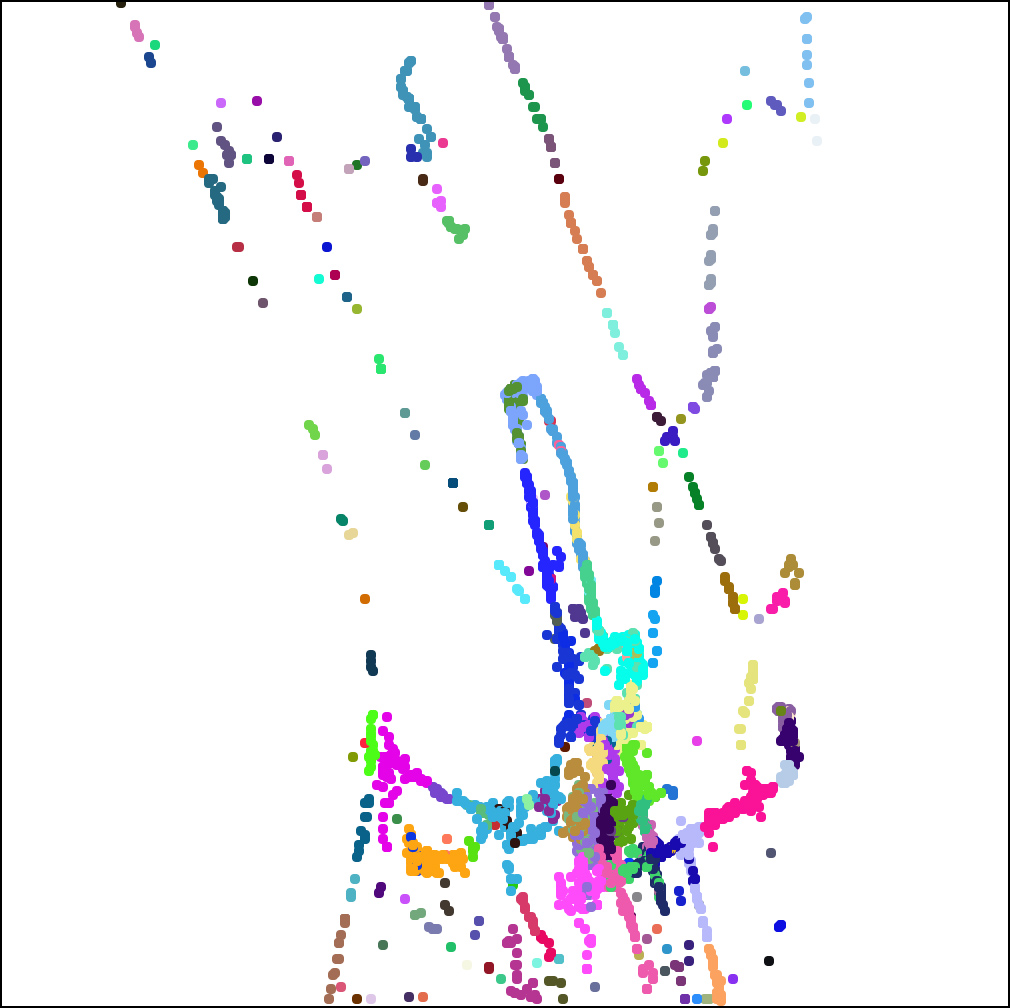
\includegraphics[scale=0.46]{Images/cities/lillehammer_groups.jpg}
%\caption{Lillehammer}
%\label{fig:lillehammer_topo}
%\end{figure}
%
%The computation results of Lillehammer can be seen in figure \ref{fig:lillehammer_topo}.
%The topology is of medium density, consisting of 4990 APs, and is 2572 meters high 
%and 8418 meters wide. From the tight clusters in the middle it is easy to make out the city centre.
%We can clearly see different groups with different sizes. Some of the smallest groups
%are highly likely so small because the distance to other nodes is too high for
%the group to hear. In the denser areas they are occasionally very
%entangeled, and it can be hard to make out the group borders.
%
%Another thing to notice is that APs are nearly always placed in straight lines.
%The straight lines are roads, and as Wigle collects data based on triangulation, the nodes
%that is only seen once will get the position they are observed in, and not an actual
%triangulated position. 
%\subsubsection{Tynset}
%The computation results of Tynset can be seen in figure \ref{fig:tynset_topo}. 
%The topology consists of 726 APs, is 1670 meters high and  6720 meters wide. 
%Unsurprisingly it resembles Lillehammer on a smaller scale.
%Again we see
%some very clearly defined groups, but in the city centre there are groups
%which overlaps. We can also see nodes that are alone in their group,
%because they are too far away from anyone else.
%Much like Lillehammer, this topology is also strongly affected by the weak
%
%triangulation of the APs, so most APs seems to be placed on top of a road. 
%
%\begin{figure}
%\center
%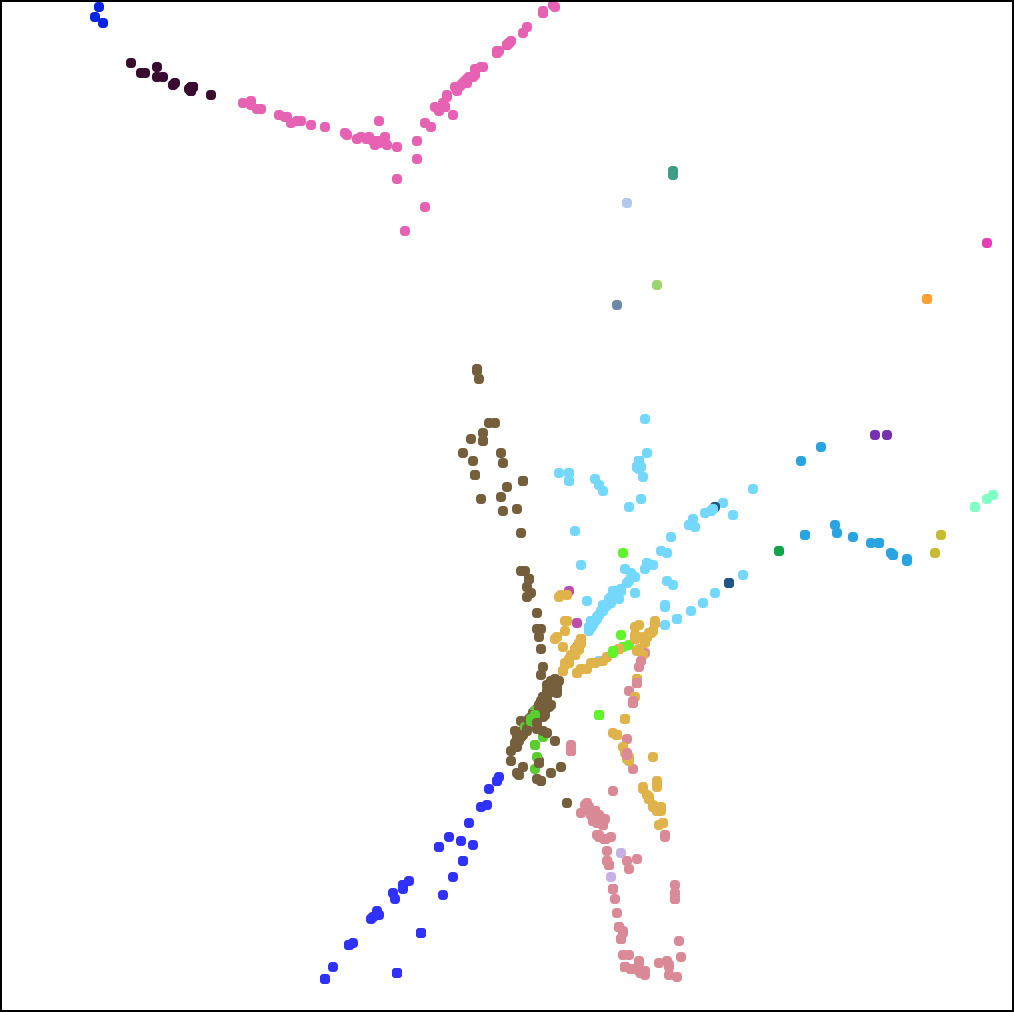
\includegraphics[scale=0.46]{Images/cities/tynset_groups.jpg}
%\caption{Tynset}
%\label{fig:tynset_topo}
%\end{figure}
%
%\subsubsection{Forks}
%
%The computation results of Forks can be seen in figure \ref{fig:forks_topo}. 
%The topology consists of 1715 nodes, and is 2122 meters high and 4495 meters wide. It
%is important to include, because it is quite different from the other topologies and
%represents a variation from the typical town and city structure of Norway.
%The size of the groups are a little more uniform when comparing it to the others.
%This can explained by the the smaller area the town is contained within. When a group
%is not full, it will almost always hear someone that it can merge with.
%We still have groups overlapping each other in the denser regions in Forks as well. 
%What is worth noticing is that the APs are positioned more realistically as locations
%of households. American towns looks more like a grid with roads in between households,
%which makes triangulation easy and a lot more accurate. 
%
%\begin{figure}
%\center
%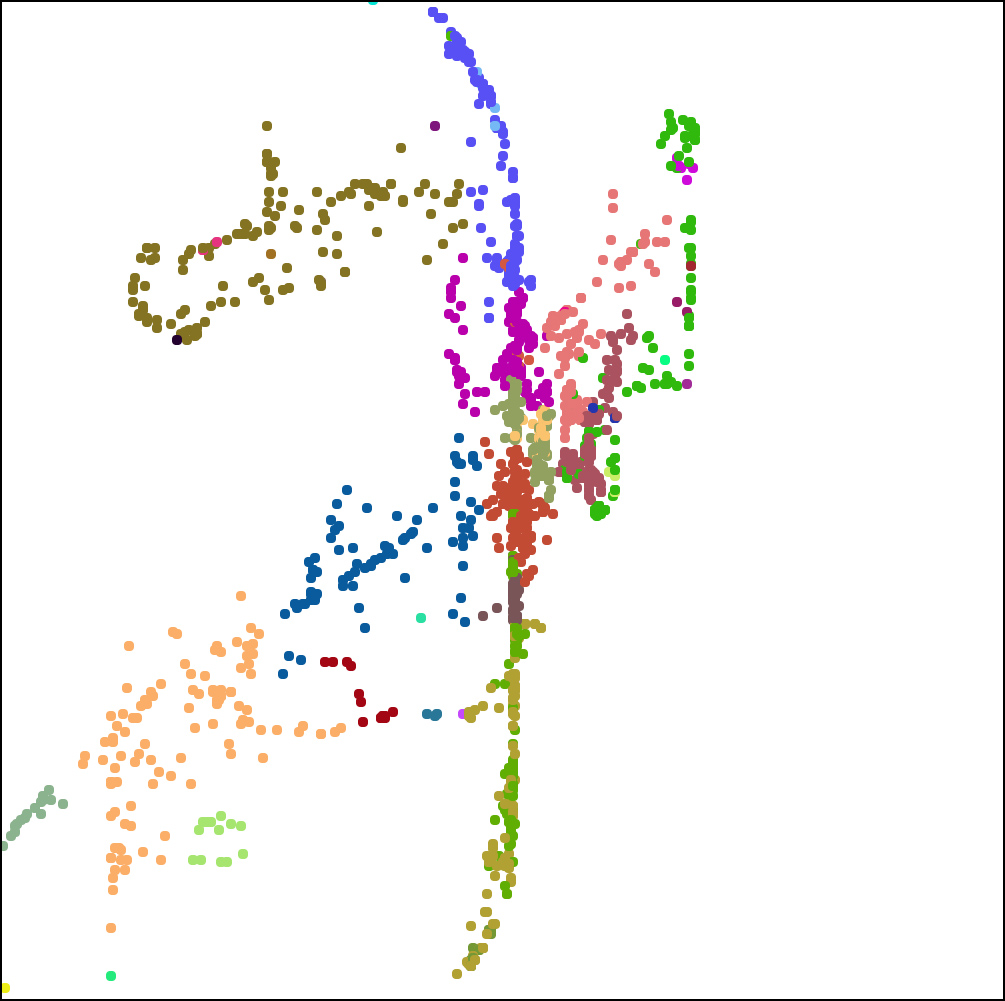
\includegraphics[scale=0.46]{Images/cities/forks_groups.jpg}
%\caption{Forks}
%\label{fig:forks_topo}
%\end{figure}
%
%
%
%
